% Options for packages loaded elsewhere
\PassOptionsToPackage{unicode}{hyperref}
\PassOptionsToPackage{hyphens}{url}
%
\documentclass[
  english,
  ,man,floatsintext]{apa6}
\usepackage{lmodern}
\usepackage{amssymb,amsmath}
\usepackage{ifxetex,ifluatex}
\ifnum 0\ifxetex 1\fi\ifluatex 1\fi=0 % if pdftex
  \usepackage[T1]{fontenc}
  \usepackage[utf8]{inputenc}
  \usepackage{textcomp} % provide euro and other symbols
\else % if luatex or xetex
  \usepackage{unicode-math}
  \defaultfontfeatures{Scale=MatchLowercase}
  \defaultfontfeatures[\rmfamily]{Ligatures=TeX,Scale=1}
\fi
% Use upquote if available, for straight quotes in verbatim environments
\IfFileExists{upquote.sty}{\usepackage{upquote}}{}
\IfFileExists{microtype.sty}{% use microtype if available
  \usepackage[]{microtype}
  \UseMicrotypeSet[protrusion]{basicmath} % disable protrusion for tt fonts
}{}
\makeatletter
\@ifundefined{KOMAClassName}{% if non-KOMA class
  \IfFileExists{parskip.sty}{%
    \usepackage{parskip}
  }{% else
    \setlength{\parindent}{0pt}
    \setlength{\parskip}{6pt plus 2pt minus 1pt}}
}{% if KOMA class
  \KOMAoptions{parskip=half}}
\makeatother
\usepackage{xcolor}
\IfFileExists{xurl.sty}{\usepackage{xurl}}{} % add URL line breaks if available
\IfFileExists{bookmark.sty}{\usepackage{bookmark}}{\usepackage{hyperref}}
\hypersetup{
  pdftitle={Adults' and Children's Comprehension of Linguistic Disjunction},
  pdfauthor={Masoud Jasbi1 \& Michael C. Frank2},
  pdflang={en-EN},
  pdfkeywords={disjunction, implicature, semantics, pragmatics, logic, language, language acquisition, language comprehension, language development},
  hidelinks,
  pdfcreator={LaTeX via pandoc}}
\urlstyle{same} % disable monospaced font for URLs
\usepackage{longtable,booktabs}
% Correct order of tables after \paragraph or \subparagraph
\usepackage{etoolbox}
\makeatletter
\patchcmd\longtable{\par}{\if@noskipsec\mbox{}\fi\par}{}{}
\makeatother
% Allow footnotes in longtable head/foot
\IfFileExists{footnotehyper.sty}{\usepackage{footnotehyper}}{\usepackage{footnote}}
\makesavenoteenv{longtable}
\usepackage{graphicx,grffile}
\makeatletter
\def\maxwidth{\ifdim\Gin@nat@width>\linewidth\linewidth\else\Gin@nat@width\fi}
\def\maxheight{\ifdim\Gin@nat@height>\textheight\textheight\else\Gin@nat@height\fi}
\makeatother
% Scale images if necessary, so that they will not overflow the page
% margins by default, and it is still possible to overwrite the defaults
% using explicit options in \includegraphics[width, height, ...]{}
\setkeys{Gin}{width=\maxwidth,height=\maxheight,keepaspectratio}
% Set default figure placement to htbp
\makeatletter
\def\fps@figure{htbp}
\makeatother
\setlength{\emergencystretch}{3em} % prevent overfull lines
\providecommand{\tightlist}{%
  \setlength{\itemsep}{0pt}\setlength{\parskip}{0pt}}
\setcounter{secnumdepth}{-\maxdimen} % remove section numbering
% Make \paragraph and \subparagraph free-standing
\ifx\paragraph\undefined\else
  \let\oldparagraph\paragraph
  \renewcommand{\paragraph}[1]{\oldparagraph{#1}\mbox{}}
\fi
\ifx\subparagraph\undefined\else
  \let\oldsubparagraph\subparagraph
  \renewcommand{\subparagraph}[1]{\oldsubparagraph{#1}\mbox{}}
\fi
% Manuscript styling
\usepackage{upgreek}
\captionsetup{font=singlespacing,justification=justified}

% Table formatting
\usepackage{longtable}
\usepackage{lscape}
% \usepackage[counterclockwise]{rotating}   % Landscape page setup for large tables
\usepackage{multirow}		% Table styling
\usepackage{tabularx}		% Control Column width
\usepackage[flushleft]{threeparttable}	% Allows for three part tables with a specified notes section
\usepackage{threeparttablex}            % Lets threeparttable work with longtable

% Create new environments so endfloat can handle them
% \newenvironment{ltable}
%   {\begin{landscape}\begin{center}\begin{threeparttable}}
%   {\end{threeparttable}\end{center}\end{landscape}}
\newenvironment{lltable}{\begin{landscape}\begin{center}\begin{ThreePartTable}}{\end{ThreePartTable}\end{center}\end{landscape}}

% Enables adjusting longtable caption width to table width
% Solution found at http://golatex.de/longtable-mit-caption-so-breit-wie-die-tabelle-t15767.html
\makeatletter
\newcommand\LastLTentrywidth{1em}
\newlength\longtablewidth
\setlength{\longtablewidth}{1in}
\newcommand{\getlongtablewidth}{\begingroup \ifcsname LT@\roman{LT@tables}\endcsname \global\longtablewidth=0pt \renewcommand{\LT@entry}[2]{\global\advance\longtablewidth by ##2\relax\gdef\LastLTentrywidth{##2}}\@nameuse{LT@\roman{LT@tables}} \fi \endgroup}

% \setlength{\parindent}{0.5in}
% \setlength{\parskip}{0pt plus 0pt minus 0pt}

% \usepackage{etoolbox}
\makeatletter
\patchcmd{\HyOrg@maketitle}
  {\section{\normalfont\normalsize\abstractname}}
  {\section*{\normalfont\normalsize\abstractname}}
  {}{\typeout{Failed to patch abstract.}}
\patchcmd{\HyOrg@maketitle}
  {\section{\protect\normalfont{\@title}}}
  {\section*{\protect\normalfont{\@title}}}
  {}{\typeout{Failed to patch title.}}
\makeatother
\shorttitle{Comprehension of Linguistic Disjunction}
\keywords{disjunction, implicature, semantics, pragmatics, logic, language, language acquisition, language comprehension, language development\newline\indent Word count: 12530}
\usepackage{lineno}

\linenumbers
\usepackage{csquotes}
\usepackage{xcolor}
\ifxetex
  % Load polyglossia as late as possible: uses bidi with RTL langages (e.g. Hebrew, Arabic)
  \usepackage{polyglossia}
  \setmainlanguage[]{english}
\else
  \usepackage[shorthands=off,main=english]{babel}
\fi

\title{Adults' and Children's Comprehension of Linguistic Disjunction}
\author{Masoud Jasbi\textsuperscript{1} \& Michael C. Frank\textsuperscript{2}}
\date{}


\affiliation{\vspace{0.5cm}\textsuperscript{1} University of California, Davis\\\textsuperscript{2} Stanford University}

\abstract{
Disjunction has played a major role in advancing theories of logic, language, and cognition, featuring as the centerpiece of debates on the origins and development of logical thought. Recent studies have argued that due to non-adult-like pragmatic reasoning, preschool children's comprehension of linguistic disjunction differs from adults in two ways. First, children are more likely to interpret \emph{or} as \emph{and} (conjunctive interpretations); Second, children are more likely to consider a disjunction as inclusive (lack of exclusivity implicatures). We tested adults and children's comprehension of disjunction in existential sentences using two- and three-alternative forced choice tasks, and analyzed children's spontaneous verbal reactions prior to their forced-choice judgments. Overall our results are compatible with studies that suggest children understand the basic truth-conditional semantics of disjunction. Children did not interpret \emph{or} as \emph{and}, supporting studies that argue conjunctive interpretations are due to task demands. In addition, even though our forced-choice tasks suggest children interpreted disjunction as inclusive, spontaneous verbal reactions showed that children were sensitive to the adult-like pragmatics of disjunction. Theoretically, these studies provide evidence against previous developmental accounts, and lend themselves to two alternative hypotheses. First, that preschool children's pragmatic knowledge is more adult-like than previously assumed, but forced-choice judgments are not sensitive enough to capture this knowledge. Second, children may have the knowledge of the relevant lexical scale themselves, but be uncertain whether a new speaker also has this knowledge (mutual knowledge of the scale).
}



\begin{document}
\maketitle

\hypertarget{introduction}{%
\section{Introduction}\label{introduction}}

When introducing disjunction to students of logic, Alfred Tarski (1941) complained about the complex factors that affect its comprehension in everyday language:

\begin{quote}
\enquote{The usage of the word \emph{or} in everyday English is influenced by certain factors of a psychological character. Usually we affirm a disjunction of two sentences only if we believe that one of them is true but wonder which one. If, for example, we look upon a lawn in normal light, it will not enter our mind to say that the lawn is green or blue, since we are able to affirm something simpler, and at the same time, stronger, namely that the lawn is green. Sometimes even, we take the utterance of a disjunction as an admission by the speaker that he does not know which of the members of the disjunction is true. (Tarski, 1941, p. 21)}
\end{quote}

\textsc{speaker ignorance} is the label we use today for the implication that the speaker does not know which disjunct is true. Tarski also noted that a disjunction has at least two other implications: exclusivity and inclusivity. Suppose, \enquote{a child has asked to be taken on a hike in the morning and to a theater in the afternoon, and we reply: No, we shall go on a hike or we shall go to the theater} (Tarski, 1941, p. 20). Tarski explained that disjunction in this example is \textsc{exclusive} because \enquote{we intend to comply with only one of the two requests} and not both. However, a disjunction may also have an \textsc{inclusive} implication like the following example: \enquote{Customers who are teachers or college students are entitled to a special reduction}. Tarski explained that \emph{or} in this example is inclusive \enquote{since it is not intended to refuse reduction to a teacher who is at the same time a college student.}

Grice (1975) argued that different implications of disjunction have different sources, strengths, and theoretical status. The inclusive implication is the literal meaning encoded by the word \emph{or} (i.e.~its semantics). It is in fact a strong entailment of disjunction, whose denial would result in a contradiction (e.g.~\enquote{Bob drank tea or coffee. He drank neither in fact!}). On the other hand, exclusivity and ignorance are weaker inferences that enrich the literal meaning of \emph{or} in context (i.e.~its pragmatics). Grice called these pragmatic inferences \textsc{implicatures} and considered them deniable or defeasible (e.g.~\enquote{Bob drank tea or coffee. He drank both in fact.} or \enquote{Bob drank tea or coffee. I know which but I'm not going to tell you.}). Under the Gricean theory, ignorance and exclusivity implicatures are inferences derived from our reasoning on why the speaker said a disjunction like \enquote{A or B}, instead of a conjunction \enquote{A and B}, or just one of the disjuncts like \enquote{A}. Grice (1975) generalized and systematized Tarski's intuition that we do not say \enquote{the lawn is green or blue} because we can say \enquote{something simpler and at the same time stronger}; namely \enquote{the lawn is green}. He argued for a general communicative principle: speakers strive to be as truthful, informative, relevant, and brief as they can. Therefore, a disjunction commonly results in the inference that the speaker could not have uttered only one of the disjuncts, probably because they were uncertain about its truth (ignorance implicature). Similarly, exclusivity of a disjunction is inferred by reasoning about the speaker's choice of the connective (\emph{or} instead of \emph{and}). Going back to Tarski's example, the child's dad could have said \enquote{we are going on a hike \emph{and} we are going to the theater} if he intended to do both. He used \emph{or} instead. Assuming he knew whether he wants to do both or not, his utterance must mean he wants to do one or the other (exclusivity implicature). Within the Gricean framework, ignorance and exclusivity implications of \emph{or} are secondary defeasible inferences, derived from the interaction of its literal inclusive meaning with conversational principles.

Complexities involved in the comprehension of disjunction have consequences for developmental theories. How does this intricate semantic and pragmatic knowledge develop in humans? When do children begin to understand a disjunction? What is their early comprehension like? Do they differ significantly from adults'? Previous studies have suggested that preschool children (age 3-5 years) understand the semantics of disjunction, yet their pragmatic knowledge differ from adults in two ways. First, they are more likely to interpret \emph{or} as \emph{and} (Braine \& Rumain, 1981; Neimark, 1970; Singh, Wexler, Astle-Rahim, Kamawar, \& Fox, 2016; Tieu et al., 2017). This is often referred to as the conjunctive interpretation of disjunction. Second, preschool children are more likely to interpret a disjunction as inclusive. In other words, unlike adults, children do not compute exclusivity implicatures, and therefore consider a disjunction as felicitous when both disjuncts are true (Chierchia, Crain, Guasti, Gualmini, \& Meroni, 2001; Chierchia et al., 2004; Crain, 2008). This is often referred to as children's \enquote{lack of exclusivity implicatures}.

In the present study, we tested adults' and preschool children's comprehension of linguistic disjunction in simple existential sentences and found children's comprehension of disjunction to be much more similar to those of adults than previously suggested. We start with a broad review of the literature on children's acquisition of disjunction. Next we present three experiments that tested adults and children using two- and three-alternative forced-choice judgment tasks. Our studies also collected and categorized children's spontaneous verbal responses in the same tasks. In our analyses, we compare and contrast the results for forced-choice vs.~free-form and spontaneous responses. Finally in General Discussion, we discuss the implications of our studies for theories of semantic and pragmatic development.

\hypertarget{litreview}{%
\subsection{Previous Research}\label{litreview}}

Children's comprehension of logical connectives \emph{and} and \emph{or} have been studied within two research programs. The first program, starting in the 1960s, was inspired by Piaget's developmental theory (Inhelder \& Piaget, 1958), and focused on the emergence of logical concepts in humans. The second research program started in the late 1990s and was inspired by the Gricean theory of meaning. Rather than emphasizing conceptual development, it focused on linguistic development, separating the roles of semantics and pragmatics in language acquisition. In this section, we briefly outline some of the main findings in these two research programs.

Within the Piagetian program, researchers hypothesized that the abstract and logical notion of disjunction (i.e.~inclusive disjunction) is constructed from the more concrete concept of \enquote{choice between two options}. The prediction was that until the age of 11 (concrete operational stage), children understand a disjunction like \enquote{A or B} as \enquote{one of the two options}. This is similar to the exclusive implication of disjunction. After age 11 (formal operational stage), children start to form abstract logical concepts and interpret \enquote{A or B} as inclusive. To examine this hypothesis, researchers conducted large scale in-class tests of school children and college students (Neimark \& Slotnick, 1970; Nitta \& Nagano, 1966). Participants were presented with pictures of objects and asked to circle those described by a statement such as \enquote{not bird}, \enquote{bird and white}, \enquote{bird or white}. These studies concluded that the majority of the participants understood negation and conjunction, but only college students correctly answered statements with disjunction. They reported that participants made two types of \enquote{errors}. First across all ages, some participants interpreted disjunction as conjunction. Second, some participants interpreted disjunction as exclusive. Based on these results, Neimark (1970) concluded that a \enquote{correct} (i.e.~inclusive) understanding of disjunction only develops in the high school years and depends on the attainment of formal operations as defined in the Piagetian theory\footnote{The term \enquote{error} has different definitions in the literature on the comprehension of disjunction. Early studies considered any response other than an inclusive interpretation as erroneous. More importantly, what counted as an error was decided by researchers. Today, however, both exclusive and inclusive interpretations are considered correct and the conjunctive interpretation is more likely to be considered erroneous. Researchers also focus more on adult-like vs.~non-adult-like behavior in children rather than \enquote{erroneous} behavior. Depending on the context, a disjunction may be interpreted as exclusive, inclusive, or even conjunctive, and adults set the benchmark interpretation for children's performance in experimental tasks.}.

Further investigations suggested that the conjunctive errors may be due to the task design of in-class tests. Paris (1973) reported that in his in-class truth-judgment task, even a fifth of college students did not differentiate \emph{or} from \emph{and}, interpreting both as conjunction. He attributed these conjunctive interpretations of \emph{or} to the application of non-linguistic strategies when the task is difficult or confusing (See Clark, 1973 for a discussion of nonlinguistic strategies in child language acquisition). He explained that children in his task (as well as some adults) were probably \enquote{comparing visual and auditory information with little regard for the implied logical relationship in the verbal description.} In a disjunction such as \enquote{A or B}, participants responded with \enquote{true} if the individual disjuncts (A, B) matched the pictures and false otherwise. Such a non-linguistic \enquote{label-matching} strategy would yield correct answers for conjunction but incorrect (conjunctive) answers for disjunction. This account also explains why in Paris (1973)'s study, conjunctive readings reduced with age and why using the word \emph{either} along with \emph{or} helped reduce conjunctive interpretations further (presumably by adding an additional linguistic cue that further differentiated conjunction and disjunction).

Further evidence for the task-dependent nature of conjunctive readings or \enquote{errors} comes from \enquote{give-item} tasks. Suppes and Feldman (1969) provided children with wooden blocks of different colors and shapes and used commands such as \enquote{give the things that are round or green.} They found that depending on the exact phrasing of the command, preschool children can interpret a disjunction as exclusive or conjunctive. However, using a similar \enquote{give-item} task, Johansson and Sjolin (1975)'s did not find considerable conjunctive interpretations. They tested Swedish-speaking children's comprehension of disjunction in present tense sentences such as \enquote{Richard wants to drink lemonade or milk. Show me what he drank!} and imperative sentences such as \enquote{Put up {[}the picture of{]} the car or the doll!}. They reported that children (as young as four years of age) interpreted a disjunction as exclusive. Based on these findings, Johansson and Sjolin (1975) argued that while linguistic understanding of \emph{or} develops early as exclusive disjunction, the logical understanding of it (as inclusive disjunction) develops late.

Braine and Rumain (1981) tested participants with both a simplified replication of Suppes and Feldman (1969)'s \enquote{give-item} task and a version of what is today known as the truth value judgment task. For their replication of Suppes and Feldman (1969), they reported that both children and adults provided a \enquote{choose-one} (i.e.~exclusive) interpretation of disjunction. They did not find any conjunctive interpretations, providing even further support for the role of task design. However, this was not the case in the truth value judgment task. In this task, a puppet described the contents of four boxes, each containing four animal toys. For example, the puppet said \enquote{Either there is a horse or a duck in the box.} The first box had both animals, the second had only a horse, the third only a duck, and the last had neither. Participants were asked if the puppet was right. The results showed that adults were split between an inclusive and an exclusive interpretation of disjunction. The 7 to 10 year-olds were more likely to consider the disjunction as inclusive. However, the youngest group (5-6 years old) was most likely to interpret a disjunction similar to a conjunction: they said the puppet was right when both animals were in the box and not right or partly right if only one of the animals was in the box. Following Paris (1973), Braine and Rumain (1981) argued that in this task, younger children do not take the contribution of the connective \emph{or} into account. Instead, they use a non-linguistic strategy in which the disjunction is right if both propositions are true, partly right if only one is true, and wrong if neither is true. Braine and Rumain (1981) concluded that children's ability to interpret a disjunction in a command develops earlier than their ability to judge its truth value.

In Braine and Rumain (1981)'s judgment task, the puppet uttered a disjunction even though the content of the box was known to both the puppet and the participant (i.e.~the speaker lacked ignorance). As Tarski (1941) noted, such uses of disjunction sound odd and infelicitous. This feature may have contributed to the application of a non-linguistic strategy and resulted in conjunctive readings. Later truth value judgment studies such as Chierchia, Crain, Guasti, and Thornton (1998) controlled for this effect of disjunction by making the puppet utter disjunction as a prediction or guess for an unknown event, and let participants judge the prediction after they see the outcome. Chierchia et al. (1998) argued that in order to truly capture children's semantic competence with \emph{or}, experiments need to test its comprehension in contexts that do not invite exclusivity implicatures. These contexts include embedding \emph{or} under linguistic operators such as negation or conditionals.

Since Chierchia et al. (1998)'s arguments, numerous studies within the Gricean program have tested preschool children's comprehension of disjunction in embedded contexts as varied as negative sentences (Crain, Gualmini, \& Meroni, 2000), conditional sentences (Gualmini, Crain, \& Meroni, 2000), restriction and nuclear scope of the universal quantifier \emph{every} (Chierchia et al., 2001, 2004), nuclear scope of the negative quantifier \emph{none} (Gualmini \& Crain, 2002), restriction and nuclear scope of \emph{not every} (Notley et al., 2012a), and prepositional phrases headed by \emph{before} (Notley et al., 2012b), as well as similar environments in other languages such as Mandarin Chinese and Japanese (Goro \& Akiba, 2004; Su, 2014; Su \& Crain, 2013). These studies almost unanimously support the hypothesis that preschool children understand the semantics of disjunction and that the inclusive implication emerges earlier than the exclusive implication. However, the lack of exclusivity in early childhood stands in sharp contrast to the earlier conclusions from the give-item tasks. Since under the Gricean account, exclusivity is the result of pragmatic (scalar) implicatures, the lack of exclusivity is considered consistent with evidence from the development of quantifier implicatures \emph{some} and \emph{all} and the overall conclusion that implicatures are slow to develop in children (Barner, Brooks, \& Bale, 2011; Noveck, 2001; Papafragou \& Musolino, 2003). Methodological issues qualify this conclusion, however. As mentioned earlier, Braine and Rumain (1981) found that the same children were more likely to interpret a disjunction as exclusive in a give-item task and inclusive/conjunctive in a truth value judgment task. Therefore, truth value judgment tasks may not reveal the full picture regarding children's knowledge of exclusivity implicatures.

More recently, two truth value judgment studies reported that the majority of preschool children in their sample interpreted a disjunction similar to a conjunction (Singh et al., 2016; Tieu et al., 2017). To control for ignorance, Tieu et al. (2017) used the \enquote{prediction mode} of the Truth Value Judgment Task, in which the puppet provides a prediction or guess. Then an event occurs and participants are asked if the prediction was right. For example, there was a chicken on the screen and two toy objects, a bus and a plane. The puppet appeared on the screen and predicted that \enquote{the chicken pushed the bus or the plane}. Then the chicken pushed either one or both of the objects. Participants stamped under a happy face or a sad face on a scorecard to show whether the puppet's guess was right or wrong. They reported that unlike adults, preschool children were more likely to consider a disjunction as \enquote{right} when both disjuncts were true, rather than only one. They concluded that the majority of children in their sample, who were 3.5 to 6.6 years of age, interpreted disjunction as conjunction. They hypothesized that this conjunctive interpretation of disjunction is due to children's non-adult-like pragmatic enrichment.

However, a recent replication of Tieu et al. (2017) by Skordos, Feiman, Bale, and Barner (2020) suggests that the high rate of conjunctive interpretations were most likely due to the experimental context's lack of plausible dissent: the experiment did not provide conditions under which utterances could be deemed false plausibly. They tested preschoolers in two conditions: replication (two-alternatives) and three-alternatives. The first condition was a direct replication of Tieu et al. (2017). The three-alternatives condition provided three objects; for example a plane, a bus, and a bicycle. The reasoning was that if there are only two objects, a disjunction is trivially true, and consequently children may consider that unacceptable. The results replicated Tieu et al. (2017)'s findings in the replication condition, but showed that conjunctive interpretations of disjunction disappeared almost completely in the three-alternatives condition. Skordos et al. (2020) concluded that children's conjunctive interpretations are most likely due to non-linguistic strategies applied when they are uncertain about some aspect of the experimental task. This conclusion is similar to the conclusions of Paris (1973) and Braine and Rumain (1981) in early studies of disjunction.

\begin{longtable}[]{@{}lll@{}}
\caption{\label{tab:conclusionsReview} Summary of tasks used in previous studies and their conclusions}\tabularnewline
\toprule
\begin{minipage}[b]{0.35\columnwidth}\raggedright
Task\strut
\end{minipage} & \begin{minipage}[b]{0.40\columnwidth}\raggedright
Conclusions\strut
\end{minipage} & \begin{minipage}[b]{0.17\columnwidth}\raggedright
Representative Study\strut
\end{minipage}\tabularnewline
\midrule
\endfirsthead
\toprule
\begin{minipage}[b]{0.35\columnwidth}\raggedright
Task\strut
\end{minipage} & \begin{minipage}[b]{0.40\columnwidth}\raggedright
Conclusions\strut
\end{minipage} & \begin{minipage}[b]{0.17\columnwidth}\raggedright
Representative Study\strut
\end{minipage}\tabularnewline
\midrule
\endhead
\begin{minipage}[t]{0.35\columnwidth}\raggedright
\textbf{School test (Imperative)} \newline \textit{(e.g. Circle all that are bird or black!)}\strut
\end{minipage} & \begin{minipage}[t]{0.40\columnwidth}\raggedright
Comprehension of \emph{or} develops in high school. Before that children often interpret it as conjunction.\strut
\end{minipage} & \begin{minipage}[t]{0.17\columnwidth}\raggedright
Neimark and Slotnick (1970)\strut
\end{minipage}\tabularnewline
\begin{minipage}[t]{0.35\columnwidth}\raggedright
\textbf{School test (Truth Value Judgment)} \newline \textit{(e.g. The bird is in the nest or the shoe is on the foot.)}\strut
\end{minipage} & \begin{minipage}[t]{0.40\columnwidth}\raggedright
Children (8-14 years) as well as some adults interpret \emph{or} as a conjunction. This is likely due to task demands and application of nonlinguistic strategies.\strut
\end{minipage} & \begin{minipage}[t]{0.17\columnwidth}\raggedright
Paris (1973)\strut
\end{minipage}\tabularnewline
\begin{minipage}[t]{0.35\columnwidth}\raggedright
\textbf{Give-item} \newline \textit{(e.g. Put up the car or the doll.)}\strut
\end{minipage} & \begin{minipage}[t]{0.40\columnwidth}\raggedright
Children (4-7 years) interpret disjunction as exclusive (choose-one). The inclusive (logical) concept of disjunction develops later.\strut
\end{minipage} & \begin{minipage}[t]{0.17\columnwidth}\raggedright
Johansson and Sjolin (1975)\strut
\end{minipage}\tabularnewline
\begin{minipage}[t]{0.35\columnwidth}\raggedright
\textbf{Give-item + Truth Value Judgment} \newline \textit{(e.g. Give me all the green things or give me all the round things.)} \newline \textit{(e.g. Either there is a cat or there is a dog in the box.)}\strut
\end{minipage} & \begin{minipage}[t]{0.40\columnwidth}\raggedright
Children (5-6 years) interpret \emph{or} as exclusive in commands but ignore its contribution in truth value judgments and interpret it as a conjunction. Interpretation of disjunction in commands develops earlier than the knowledge of its truth conditions.\strut
\end{minipage} & \begin{minipage}[t]{0.17\columnwidth}\raggedright
Braine and Rumain (1981)\strut
\end{minipage}\tabularnewline
\begin{minipage}[t]{0.35\columnwidth}\raggedright
\textbf{Truth Value Judgment (controlling for Speaker Ignorance)} \newline \textit{(e.g. A troll ate a piece of pizza or an ice cream.)}\strut
\end{minipage} & \begin{minipage}[t]{0.40\columnwidth}\raggedright
Children (4-6 years) understand \emph{or} as inclusive disjunction. Two studies report majority conjunctive interpretations too.\strut
\end{minipage} & \begin{minipage}[t]{0.17\columnwidth}\raggedright
Chierchia et al. (2004), Tieu et al. (2017)\strut
\end{minipage}\tabularnewline
\begin{minipage}[t]{0.35\columnwidth}\raggedright
\textbf{Truth Value Judgment (controlling for Speaker ignorance and Number of alternatives)}\strut
\end{minipage} & \begin{minipage}[t]{0.40\columnwidth}\raggedright
Children (4-6 years) understand the truth conditions of \emph{or} similar to inclusive disjunction. No evidence for conjunctive interpretations.\strut
\end{minipage} & \begin{minipage}[t]{0.17\columnwidth}\raggedright
Skordos et al. (2020)\strut
\end{minipage}\tabularnewline
\bottomrule
\end{longtable}

To summarize, our review of previous literature suggests that the design of an experimental task can have a big impact on our conclusions about children's comprehension of disjunction (Table \ref{tab:conclusionsReview}). First, different tasks may be more or less suitable for capturing different implications of disjunction. For example, a \enquote{Give-item} task can successfully capture exclusive implications, while a TVJT task with plausible context for speaker ignorance is more successful in capturing inclusive implications. Second, regardless of task type, increased task demands or infelicitous use of disjunction can result in increased conjunctive interpretations of disjunction. With the give-item task, Suppes and Feldman (1969) found a considerable rate of conjunctive interpretations, but these interpretations disappeared in Braine and Rumain (1981)'s more simplified replication. Similarly, Tieu et al. (2017) reported that a large number of children interpreted \emph{or} as \emph{and}, but these conjunctive readings also disappeared when Skordos et al. (2020)'s replication controlled for the number of alternatives in the task. Therefore, previous studies highlight the role of task design and measurement in studying children's comprehension of disjunction. More specifically and with respect to conjunctive interpretations of disjunction, previous studies provide substantial evidence linking them to task design. While it is plausible to consider non-adult-like pragmatic computations as a cause of conjunctive readings of disjunction in children, it is important to first conclusively rule out the influence of task design.

In the studies reported here we use an experimental paradigm that avoids potential issues discovered and discussed in the previous literature. First, our experiments are presented as a guessing game in which a character guesses the animal on a card without seeing it and participants decide if the guess is right. This way the experimental context eliminates the issue of speaker ignorance by making it part of the game. Second, the card game involves three alternative animals (cat, dog, and elephant) which allows for a disjunction guess such as \enquote{cat or dog} to be plausibly false when the card has an elephant. Third, our paradigm uses declarative sentences as guesses and avoids imperatives which can lead to more complex implications. Fourth, our studies explicitly test children's strategies using both binary and ternary forced choice tasks, which allows children to provide more nuanced responses to linguistic stimuli. Katsos and Bishop (2011) was the first study to use binary as well as ternary tasks for assessing scalar implicatures in children's comprehension. They reported that when the quantifier \emph{some} was used infelicitously in contexts where \emph{all} would have been more appropriate, the ternary task reflected this infelicity judgment better (children were more likely to pick the intermediate option) than the binary task. We similarly included a ternary forced-choice task to see if the intermediate response option can be successful in capturing the exclusivity implicature of disjunction. Previous studies avoided one or the other of these potential issues but to our knowledge the experiments presented here are the first to avoid them all, providing a better assessment of children's underlying competence with linguistic disjunction.

\hypertarget{present-studies}{%
\subsection{Present Studies}\label{present-studies}}

The goal of this study was to further simplify task design and measure children's comprehension of disjunction in multiple ways. We used existential sentences (e.g.~\emph{there is a cat or a dog}) in the context of a simple card game. The game controlled for the effect of speaker ignorance/knowledge by making the speaker guess what was on a card without seeing it. The study included trials with the word \emph{and} to control for the comprehension of conjunction in the same task. The study also had adult participants as controls for children's performance in the task. Children's comprehension was measured in three different ways: a two-alternative forced choice task (2AFC), a three-alternative forced choice task (3AFC), and the analysis of children's spontaneous verbal reactions before they made their forced-choice judgments. Table \ref{tab:study1info} provides the summary of methods used in Experiments 1, 2, and 3.

\begin{longtable}[]{@{}lllll@{}}
\caption{\label{tab:study1info}Summary of Experiment 1, 2 and 3 methods}\tabularnewline
\toprule
\begin{minipage}[b]{0.16\columnwidth}\raggedright
Study\strut
\end{minipage} & \begin{minipage}[b]{0.01\columnwidth}\raggedright
N\strut
\end{minipage} & \begin{minipage}[b]{0.17\columnwidth}\raggedright
Age\strut
\end{minipage} & \begin{minipage}[b]{0.17\columnwidth}\raggedright
Mode\strut
\end{minipage} & \begin{minipage}[b]{0.34\columnwidth}\raggedright
Response Options\strut
\end{minipage}\tabularnewline
\midrule
\endfirsthead
\toprule
\begin{minipage}[b]{0.16\columnwidth}\raggedright
Study\strut
\end{minipage} & \begin{minipage}[b]{0.01\columnwidth}\raggedright
N\strut
\end{minipage} & \begin{minipage}[b]{0.17\columnwidth}\raggedright
Age\strut
\end{minipage} & \begin{minipage}[b]{0.17\columnwidth}\raggedright
Mode\strut
\end{minipage} & \begin{minipage}[b]{0.34\columnwidth}\raggedright
Response Options\strut
\end{minipage}\tabularnewline
\midrule
\endhead
\begin{minipage}[t]{0.16\columnwidth}\raggedright
Experiment 1\strut
\end{minipage} & \begin{minipage}[t]{0.01\columnwidth}\raggedright
57\strut
\end{minipage} & \begin{minipage}[t]{0.17\columnwidth}\raggedright
Adults\strut
\end{minipage} & \begin{minipage}[t]{0.17\columnwidth}\raggedright
Online (Mturk)\strut
\end{minipage} & \begin{minipage}[t]{0.34\columnwidth}\raggedright
Wrong, Right\strut
\end{minipage}\tabularnewline
\begin{minipage}[t]{0.16\columnwidth}\raggedright
\strut
\end{minipage} & \begin{minipage}[t]{0.01\columnwidth}\raggedright
52\strut
\end{minipage} & \begin{minipage}[t]{0.17\columnwidth}\raggedright
Adults\strut
\end{minipage} & \begin{minipage}[t]{0.17\columnwidth}\raggedright
Online (Mturk)\strut
\end{minipage} & \begin{minipage}[t]{0.34\columnwidth}\raggedright
Wrong, Kinda Right, Right\strut
\end{minipage}\tabularnewline
\begin{minipage}[t]{0.16\columnwidth}\raggedright
Experiment 2\strut
\end{minipage} & \begin{minipage}[t]{0.01\columnwidth}\raggedright
42\strut
\end{minipage} & \begin{minipage}[t]{0.17\columnwidth}\raggedright
3;1-5;2, M=4;3\strut
\end{minipage} & \begin{minipage}[t]{0.17\columnwidth}\raggedright
Preschool Experiment Room\strut
\end{minipage} & \begin{minipage}[t]{0.34\columnwidth}\raggedright
Circle (Wrong), Little Star (Little Right), Big Star (Right) + Open-ended Feedback\strut
\end{minipage}\tabularnewline
\begin{minipage}[t]{0.16\columnwidth}\raggedright
Experiment 3\strut
\end{minipage} & \begin{minipage}[t]{0.01\columnwidth}\raggedright
50\strut
\end{minipage} & \begin{minipage}[t]{0.17\columnwidth}\raggedright
3;6-5;9, M=4;7\strut
\end{minipage} & \begin{minipage}[t]{0.17\columnwidth}\raggedright
Preschool Experiment Room\strut
\end{minipage} & \begin{minipage}[t]{0.34\columnwidth}\raggedright
Yes (Right), No (Wrong) + Open-ended Feedback\strut
\end{minipage}\tabularnewline
\bottomrule
\end{longtable}

\hypertarget{study1}{%
\section{Experiment 1: Adult 2AFC and 3AFC Judgments}\label{study1}}

This study examines adults' comprehension of \emph{or}, and uses it as a benchmark for children's comprehension in Experiments 2 and 3. We tested adults in both two-alternative and three-alternative forced choice tasks (2AFC and 3AFC).

\hypertarget{methods}{%
\subsection{Methods}\label{methods}}

\hypertarget{participants}{%
\subsubsection{Participants}\label{participants}}

109 English speaking adults participated via Amazon Mechanical Turk (MTurk). 57 of them were assigned to a 2AFC judgment task and 52 to a 3AFC judgment task. In the 2AFC task, participants had to judge using the options \enquote{wrong} and \enquote{right}. In the 3AFC task they had to choose between \enquote{wrong}, \enquote{kinda right}, and \enquote{right}\footnote{There are many possible labels for the middle option on a scale, including \enquote{kinda right}, \enquote{kinda wrong}, or \enquote{neither}. A later experiment, tested different intermediate labels and found that adults consider \enquote{kinda right} to be a more suitable option for capturing pragmatic infelicities (see Jasbi, Waldon, \& Degen, 2019). We expect similar behavior from labels that refer to non-maximal degrees of being \enquote{right} such as \enquote{a bit right} or \enquote{a little right}.}. The two conditions were otherwise identical. The task took about 5 minutes on average to complete. At the end of the study, participants received \$0.4 as compensation. All participants provided informed consent before taking the experiment.

\hypertarget{stimuli}{%
\subsubsection{Stimuli}\label{stimuli}}

We used six images of cards, each with one or two cartoon animals on them. Three cards had one animal and three cards had two (Figure \ref{fig:stimuli} in Appendix). We represent these six cards with animal names in small caps: \textsc{cat, dog, ele, cat+dog, cat+ele, dog+ele} (\textsc{ele} stands for elephant). In each trial, a card was shown to the participant and a blindfolded cartoon character guessed what animal was on the card. The guess was either a simple existential sentence (\emph{There is a cat}, \emph{There is a dog}, \emph{There is an elephant}), a conjunction (e.g.~\emph{There is a cat and a dog}, \emph{There is a cat and an elephant}, \emph{There is a dog and an elephant}), or a disjunction (\emph{There is a cat or a dog}, \emph{There is a cat or an elephant}, \emph{There is a dog or an elephant}). Crossing different cards and guesses results in 54 different possible trials. However, not all these trials are equally informative for our purposes so we created 8 trial types that balanced the number of animals on the cards (one vs.~two), types of guesses (simple, conjunction, disjunction), as well as (expected) true vs.~false guesses. Figure \ref{fig:trialtypes} shows our trial types using example cards as rows and example utterances as columns.

Control trials consisted of simple guesses (e.g.~\emph{elephant}, \emph{cat}) with cards that had one animal (e.g.~\textsc{cat}) or two animals (e.g.~\textsc{cat+dog}). In half of these trials the description was true and in half it was false. When two animals were on the card (e.g.~\textsc{cat+dog}) and one was guessed (e.g.~\emph{cat}), the guess could be infelicitous or even false if interpreted exhaustively (e.g.~\textbf{only} \emph{cat}). In addition to acting as a control, such trials could show how often children derive exhaustive implicatures. Conjunction trials (e.g.~\emph{cat and dog}) were controls for disjunction trials. Conjunction trials were false when only one animal was on the card and true when both were. Finally, disjunction trials constituted the critical trials of our experiments. When only one animal was on the card (e.g.~\textsc{cat}) the disjunction guess (e.g.~\emph{cat or dog}) was true. When two animals were on the card (e.g.~\textsc{cat+dog}), the disjunction guess (e.g.~\emph{cat or dog}) could be judged as true but infelicitous or even false. Such disjunction trials help us understand whether participants interpreted disjunction as inclusive or exclusive.

We should emphasize that throughout this paper we use example cards (\textsc{cat} and \textsc{cat+dog}) as well as example utterances (\emph{elephant}, \emph{cat}, \emph{cat and dog}, \emph{cat or dog}) to represent trial types. For example, the \enquote{simple true} trial-type represented by the card \textsc{cat} and the utterance \emph{cat}, includes similar trials with the card \textsc{dog} and the guess \emph{dog}, as well as the card \textsc{ele} and the guess \emph{elephant}. Participants saw trials instantiated with all of the different cards and utterances, however, and trials were created randomly for each participant. We also use the short forms \emph{cat}, \emph{cat and dog}, and \emph{cat or dog} without the existential carrier phrase \emph{there is} to represent the guesses in this paper.

\begin{figure}

{\centering 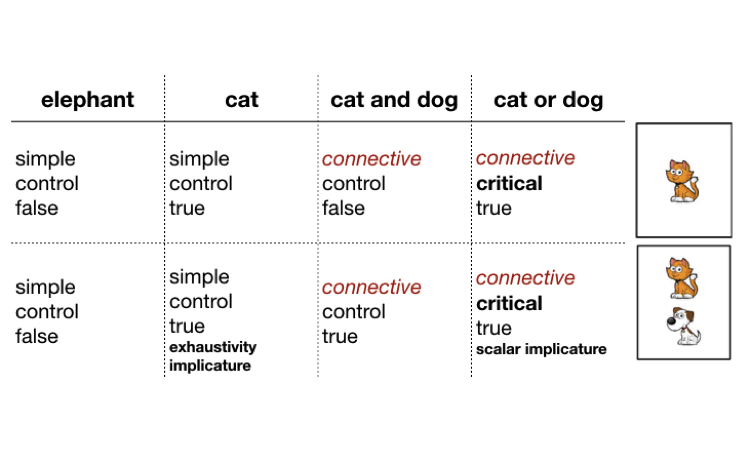
\includegraphics{Jasbi-Frank-2019_files/figure-latex/trialtypes-1} 

}

\caption{Rows show example cards and columns example utterances (guesses). Each cell represents a trial type.}\label{fig:trialtypes}
\end{figure}

\hypertarget{procedure}{%
\subsubsection{Procedure}\label{procedure}}

The experiment had three phases: introduction, instruction, and test. In the introduction, participants saw the six cards and read that they would play a guessing game. Then a blindfolded cartoon character named Bob appeared on the screen. Participants were told that in each round of the game, they would see a card and Bob was going to guess what animal was on the card. The study emphasized that Bob could not see anything. Participants were asked to judge whether Bob's guess was right. In the instruction phase, participants saw an example trial where a card with the image of a dog was shown with the following sentence written above Bob's head: \emph{There is a cat on the card}. All participants correctly responded with \enquote{wrong} and proceeded to the test phase. In the test phase, participants saw one trial per trial type. Within each trial type, the specific card and guess were chosen at random. The order of trial types was also randomized. Figure \ref{fig:stimuli} in the appendix shows an example test trial.

\hypertarget{results}{%
\subsection{Results}\label{results}}

\begin{figure}
\centering
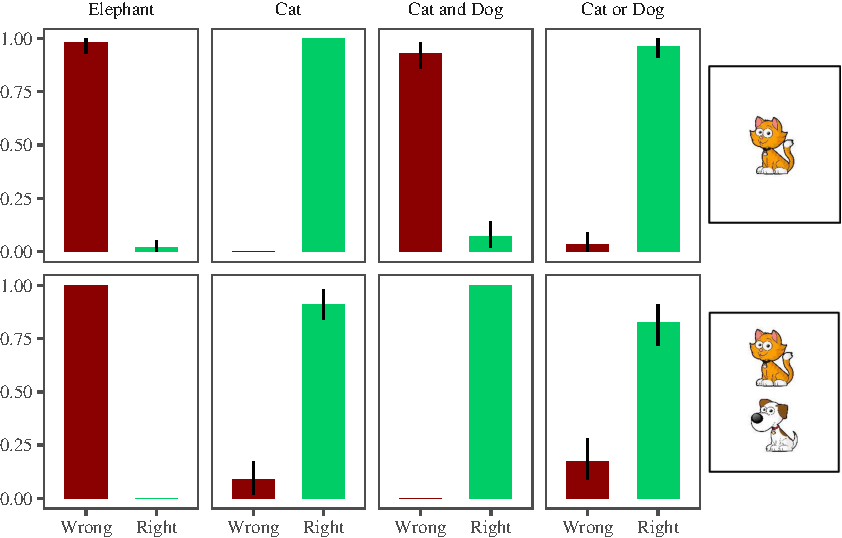
\includegraphics{Jasbi-Frank-2019_files/figure-latex/binaryAdultsPlot-1.pdf}
\caption{\label{fig:binaryAdultsPlot}Adults' two-alternative forced choice judgments in Experiment 1. Columns represent example guesses and rows example cards.}
\end{figure}

Figure \ref{fig:binaryAdultsPlot} shows the results for the adult 2AFC task. Starting with the leftmost column, participants judged false simple trials as \enquote{wrong}. In such trials the guessed animal (e.g.~\emph{elephant}) was not on the card. In true simple and true-but-incomplete simple trials, the guessed animal (e.g.~\emph{cat}) was on the card and participants judged the guess \enquote{right}. Moving to connective trials, when a conjunction (e.g.~\emph{cat and dog}) was false (i.e.~only one animal was on the card) participants judged the guess \enquote{wrong}. When the conjunction was true (i.e.~both animals were on the card) they judged it \enquote{right}. Both true disjunction trials and true-but-infelicitous disjunction trials were judged as \enquote{right}. A disjunction guess (e.g.~\emph{cat or dog}) was true when one of the animals was on the card (e.g.~\textsc{cat}) and true-but-infelicitous when both were (e.g.~\textsc{cat+dog}).

\begin{figure}
\centering
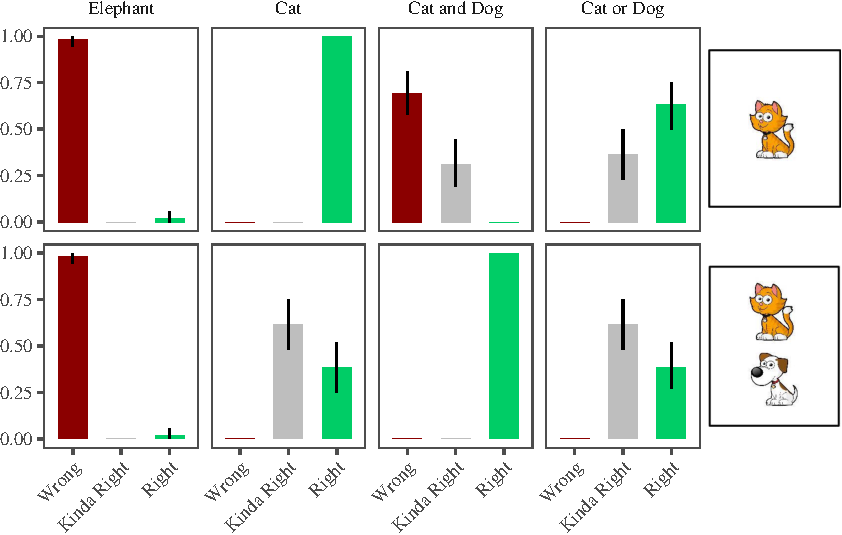
\includegraphics{Jasbi-Frank-2019_files/figure-latex/ternaryAdultsPlot-1.pdf}
\caption{\label{fig:ternaryAdultsPlot}Adults' three-alternative forced choice judgments in Experiment 1.}
\end{figure}

Figure \ref{fig:ternaryAdultsPlot} shows the results for the 3AFC judgment task. The addition of an intermediate response option did not affect false simple, true simple, and true conjunction trials. In false simple trials, the animal mentioned (e.g.~\emph{elephant}) was not on the card, and participants judged the guess \enquote{wrong}. In true simple trials the animal mentioned (e.g.~\emph{cat}) was the only animal on the card and participant considered the guess \enquote{right}. This was similar to true conjunction trials in which two animals were on the card (e.g.~\textsc{cat+dog}) and the guess mentioned both (e.g.~\emph{cat and dog}). Participants judged true conjunction trials as \enquote{right} in both 2AFC and 3AFC tasks.

Four trial types showed different patterns of judgments in the 2AFC and the 3AFC tasks. In true-but-incomplete simple trials, one animal was mentioned (e.g.~\emph{cat}) but two animals were on the card (e.g.~\textsc{cat+dog}). Participant judgments were divided between \enquote{right} and \enquote{kinda right} options. In false conjunction trials, only one animal was on the card (e.g.~\textsc{cat}), but two animals were guessed (e.g \emph{cat and dog}). Most adults considered such false conjunctions \enquote{wrong} but some chose \enquote{kinda right}. The intermediate option may have been used to express partial truth of the guess because one of the guessed animals was on the card. With true disjunction and true-but-infelicitous disjunction guesses, responses were split between \enquote{kinda right} and \enquote{right}. It is likely that participants had different reasons for choosing \enquote{kinda right} in each disjunction trial type. In true disjunction trials, participants may have considered a simple guess (e.g.~\emph{there is a cat}) as more appropriate. In true-but-infelicitous trials, participants may have expected the connective \emph{and} instead of \emph{or}. As we shall see in the next two experiments, children explicitly mention these alternatives in their open-ended (free-form) responses. Since we are mainly interested in the differences between adults and children, we defer statistical analysis to Experiment 2 where we compare children and adults responses.

\hypertarget{discussion}{%
\subsection{Discussion}\label{discussion}}

\begin{longtable}[]{@{}lllll@{}}
\caption{\label{tab:truthtable} Truth conditions of conjunction, inclusive disjunction, and exclusive disjunction. \enquote{cat} and \enquote{dog} represent the propositions that \enquote{there is a cat on the card} and \enquote{there is a dog on the card} respectively.}\tabularnewline
\toprule
cat & dog & cat \(\land\) dog & cat \(\lor\) dog & cat \(\oplus\) dog\tabularnewline
\midrule
\endfirsthead
\toprule
cat & dog & cat \(\land\) dog & cat \(\lor\) dog & cat \(\oplus\) dog\tabularnewline
\midrule
\endhead
T & T & T & T & F\tabularnewline
T & F & F & T & T\tabularnewline
F & T & F & T & T\tabularnewline
F & F & F & F & F\tabularnewline
\bottomrule
\end{longtable}

Consider the truth conditions for conjunction and disjunction in classical logic shown in Table \ref{tab:truthtable}. A conjunction is true when both conjuncts are true and false otherwise. An inclusive disjunction is true when at least one disjunct is true, and false otherwise. An exclusive disjunction is true when only one of the disjuncts is true and false otherwise. Let's also assume a simple linking function in which false statements map to \enquote{wrong} and true statements to \enquote{right.}\footnote{see Jasbi et al. (2019) for a discussion of linking assumptions in forced-choice truth-value judgment tasks.} In the 2AFC task, judgments for \emph{and} matched logical conjunction and \emph{or} inclusive disjunction. If adults in our task interpreted \emph{or} as exclusive, we expected majority \enquote{wrong} responses when both disjuncts were true. This is not what we found.

If truth conditions were all that mattered, the addition of the intermediate option (kinda right) in the 3AFC task should not have substantially affected the judgments. In fact it did not in false simple trials, true simple trials, and true conjunction trials. These cases showed unequivocal \enquote{wrong} and \enquote{right} judgments. But in four other trial types, the intermediate option (kinda right) reflected more graded judgments. These trial-types represented utterances that were false, had false implications, or were sub-optimal as guesses.

First, responses in the false conjunction trials were split between \enquote{wrong} and \enquote{kinda right} responses. In such trials, even though the guess was false, it was not completely incorrect; one of the animals was guessed correctly. Therefore, choosing the intermediate option could reflect the judgment that such guesses are better than those that fail to name any animal on the card. In the other three trial types, responses were split between \enquote{kinda right} and \enquote{right} responses. In true-but-incomplete simple trials (e.g.~\emph{cat} as guess and \textsc{cat+dog} as card), as well as true-but-infelicitous disjunction trials (e.g.~\emph{cat or dog} as guess and \textsc{cat+dog} as card), the utterances were literally true but carried defeasible false implicature; more specifically, in true-but-incomplete simple trials the exhaustive implicature (e.g.~\enquote{only a cat is on the card}) and in true-but-infelicitous disjunction trials the exclusivity implicature (e.g.~\enquote{there is a cat or a dog, but not both}). In both these cases, a conjunction (e.g.~\emph{cat and dog}) was the optimal guess and participants' choice of the middle option \enquote{kinda right} likely reflected this judgment as reaction towards the defeasible false implicature. Finally, when only one animal was on the card (e.g.~\textsc{cat}), a disjunction guess (e.g.~\emph{cat or dog}) was literally true but sub-optimal as a guess. A simple guess (e.g.~\emph{cat}) would have been better. Therefore, disjunction guesses (with either one or both disjuncts being true) had intermediate acceptability.

In a forced choice task, participants may differ on how they respond to cases of intermediate acceptability. Some may decide to ignore the slight unacceptability and focus on the truth of the statement. Others may decide to focus on the fact that a better guess was not made and express this in their judgments. This decision is independent of a participant's judgment of the linguistic stimuli, and depends on several factors including what matters for the purposes of the task and what type of measurement is used. For example, in a two-alternative task, most adults may not consider non-truth-conditional violations grave enough to render a guess as \enquote{wrong}. Therefore, judgments in a 2AFC task match the truth of a guess. However, if a third intermediate option is provided, participants may opt to also express the incompleteness or infelicity of a guess in the task - depending on the label of the intermediate option. In a followup study, we found that participants opt for the intermediate option more often if it is labeled as \enquote{kinda right} rather than \enquote{neither} (Jasbi et al., 2019). Most importantly, children may differ from adults in how they approach intermediate judgments in forced choice tasks. This source of variation between children and adults has remained relatively unexplored, despite previous evidence and arguments for it (Katsos, 2014; Katsos \& Bishop, 2011). The next two experiments provide evidence that children may differ from adults in how they deal with the intermediate acceptability of disjunction.

We should add here that we are aware of one previous study similar to the one presented here on adults' comprehension of disjunction in simple existential sentences using pictures and forced-choice judgments. Chevallier et al. (2008) presented participants with words (e.g.~TABLE), pseudo-words (e.g.~JAMIS), or non-words (e.g.~RSOUB) as well as statements about their spelling containing disjunctions such as \enquote{there is an A or a B} (in the word). Participants responded with \enquote{true}/\enquote{false} in a binary task. Even though they used different response options to ours and they were more concerned with response times and processing of implicatures, they reported similar results to the ones presented in our study. Most importantly, participants accepted a disjunction when both disjuncts were true 50-80\% of the time depending on how much time they were given to respond. The higher end of this range is consistent with the findings of our binary task and the lower end is consistent with the results of our ternary task which showed more sensitivity to pragmatic inferences. We should emphasize that the most important difference between Chevallier et al. (2008)'s study and ours is that we controlled for the role of speaker ignorance in our paradigm by presenting the task as a guessing game.

\hypertarget{study2}{%
\section{Experiment 2: Children's 3AFC judgments and open-ended feedback}\label{study2}}

This experiment tested children's comprehension of disjunction in the same guessing game and compared them to those of adults'. Since the 3AFC judgment task in Experiment 1 was better at capturing the nuances of adults' pragmatic reasoning, we decided to first test children with the 3AFC task. We also provide an analysis of children's open-ended and spontaneous verbal reactions to the guesses before they made their forced choice judgments.

\hypertarget{methods-1}{%
\subsection{Methods}\label{methods-1}}

\hypertarget{participants-1}{%
\subsubsection{Participants}\label{participants-1}}

We recruited 42 English speaking children from the Bing Nursery School at Stanford University. Children were between 3;1 and 5;2 years old (mean = 4;3). Parents of children had provided written informed consent for this experiment.

\hypertarget{materials}{%
\subsubsection{Materials}\label{materials}}

We used the same set of cards and linguistic stimuli as the ones in Experiment 1. There were 8 trial types and 2 trials per trial type for a total of 16 trials. We made two changes to make the experiment more suitable for children. First, instead of the fictional character Bob, a puppet named Jazzy played the guessing game with them. Jazzy wore a sleeping mask over his eyes during the game (Figure \ref{fig:stimuli}). Second, a pilot study showed that a scale with three alternatives is better understood and used by children if it is presented in the form of rewards to the puppet rather than verbal responses such as \enquote{wrong}, \enquote{a little bit right}, and \enquote{right}, or even hand gestures such as thumbs up, middle, and down. Therefore, we placed a set of red circles, small blue stars, and big blue stars in front of the children. These tokens were used to reward the puppet after each guess. During the introduction, the experimenter explained that if the puppet was right, the child should give him a big star; if the puppet was a little bit right, a little star, and if he was not right, a red circle.

\hypertarget{procedure-1}{%
\subsubsection{Procedure}\label{procedure-1}}

The experiment was carried out in a quiet room with a small table and two small chairs. Children sat on one side of the table and the experimenter and the puppet on the other side facing the children. The groups of circles, small stars, and big stars were placed in front of the child from left to right respectively. A deck of six cards was in front of the experimenter. Similar to study 1 with adults, study 2 had three phases: introduction, instruction, and test.

The goal of the introduction was for the experimenter to show the cards to the children and make sure they recognized the animals and knew their names. The experimenter showed the cards to the children and asked them to label each animal. All children recognized the animals and could label them correctly. In the instruction phase, children went through three example trials. The experimenter explained that he was going to play with the puppet first, so that the child could learn the game. He removed the six introduction cards and placed a deck of three cards face-down on the table. From top to bottom (first to last), the cards had the following images: \textsc{cat}, \textsc{ele}, \textsc{cat+dog} (Table \ref{tab:instruction}). The experimenter put the sleeping mask on the puppet's eyes and explained that the puppet is going to guess what animal is on the cards. He then picked the first card and asked the puppet: \enquote{What do you think is on this card?} The puppet replied with \enquote{\emph{There is a dog}}. The experimenter showed the \textsc{cat}-card to the child and explained that when the puppet is \enquote{not right} he gets a circle\footnote{The pilot study had shown that some children struggle with understanding the word \enquote{wrong}, so \enquote{not right} was used instead.}. He then asked the child to give the puppet a circle. Rewards were collected by the experimenter and placed under the table to not distract the child. The second trial followed the same pattern except that the puppet guessed \enquote{right} and the experimenter invited the child to give the puppet a big star. In the final trial of the instruction, the puppet guessed that \enquote{\emph{there is a cat}} on the card when the card was \textsc{cat+dog}. The experimenter said that the puppet was \enquote{a little right} and asked the child to give him a little star.

In the test phase, the experimenter removed the three instruction cards and placed a deck of 16 randomized cards on the table. He explained that it was the child's turn to play with the puppet. For each card, the puppet provided a guess and the child provided the puppet with a reward. The guesses were paired with each card in a way that allowed two trials per 8 trial types\footnote{A more detailed description of the procedure as well as the randomization code for the test phase is available on the study's online repository.}.

\hypertarget{feedbackCoding}{%
\subsubsection{Offline Annotations}\label{feedbackCoding}}

While playing the game, children often provided spontaneous verbal feedback or reactions to the puppet's guesses. For example if the puppet guessed \enquote{\emph{there is a cat}} and they saw the \textsc{dog} card, children said (even shouted): \enquote{\emph{No! Dog!}}. These reactions happened naturally before children provided their forced-choice responses by giving the puppet a circle, a little star, or a big star. These verbal responses were categorized into four types based on what words children produced: 1. None, 2. Judgments, 3. Descriptions, and 4. Corrections. The first category (none) referred to cases where children did not say anything (only rewarded the puppet). The second category (judgments) referred to positive/negative words that did not include the name of the animals on the card, for example: \enquote{you are right!}, \enquote{yes}, \enquote{nope}, or \enquote{you winned!}. In the third category (descriptions), children mentioned the name of the animal(s) on the card: \enquote{cat!}, \enquote{dog and elephant!}, \enquote{There is a cat and a dog!} etc. Finally, with correction, children added extra focus and functional elements such as focus words \emph{just}, \emph{only}, or stressed the connective word \emph{AND}. Examples include: \enquote{Just a cat!}, \enquote{Both!}, \enquote{The two are!}, \enquote{Only cat!}, \enquote{cat AND dog} (with emphasis placed on \emph{and}). In trials where the child provided both judgments as well as descriptions or corrections (e.g.~\enquote{Yes! Cat!}), we placed the feedback into the more informative categories, namely description or correction. We should emphasize that the annotation of children's spontaneous verbal feedback was independent of whether the guess was normatively considered \enquote{right} or \enquote{wrong} and relied only on the words they produced.

\hypertarget{results-1}{%
\subsection{Results}\label{results-1}}

\hypertarget{three-alternative-forced-choice-judgments}{%
\subsubsection{Three-Alternative Forced-Choice Judgments}\label{three-alternative-forced-choice-judgments}}

\begin{figure}
\centering
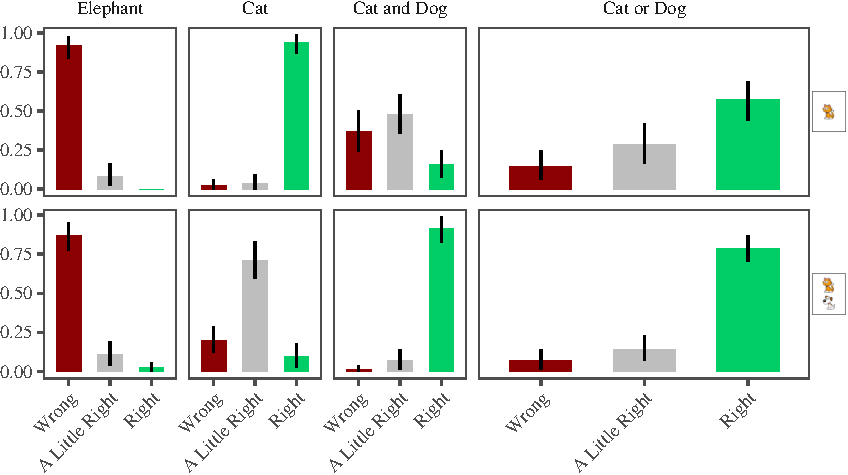
\includegraphics{Jasbi-Frank-2019_files/figure-latex/childrenTernaryPlot-1.pdf}
\caption{\label{fig:childrenTernaryPlot}Children's three-alternative forced-choice judgments in Experiment 2.}
\end{figure}

Figure \ref{fig:childrenTernaryPlot} shows the results for children's 3AFC judgments. Starting with the leftmost column in Figure \ref{fig:childrenTernaryPlot}, children judged false simple trials as \enquote{wrong}. In these trials the mentioned animal (e.g.~\emph{elephant}) was not on the card. Moving to the second column, children judged true simple trials as \enquote{right}. In these trials the mentioned animal (e.g.~\emph{cat}) was the only animal on the card. Here we ignore the results for true-but-incomplete trials in which the animal mentioned (e.g.~\emph{cat}) was only one of the animals on the card (e.g.~\textsc{cat+dog}). The reason is that such trials were used in the instruction phase to introduce the \enquote{little bit right} option, and the results are probably biased by the instructions. However, it is important to note that the instruction was successful and the majority of children considered such guesses as \enquote{kinda right}.

Moving to the third column, children judged false conjunction trials as \enquote{wrong} or \enquote{a little right}. In these trials, only one animal was on the card (e.g.~\textsc{cat}), but two were mentioned (e.g.~\emph{cat and dog}). In true conjunction trials, both mentioned animals were on the card and children judged the guess as \enquote{right}. Finally, in true disjunction trials only one animal was on the card and children considered the guess (e.g.~\emph{cat or dog}) as either \enquote{right} or \enquote{kinda right}. In true-but-infelicitous disjunction trials both animals were on the card and children judged the disjunction \enquote{right}.

\begin{figure}
\centering
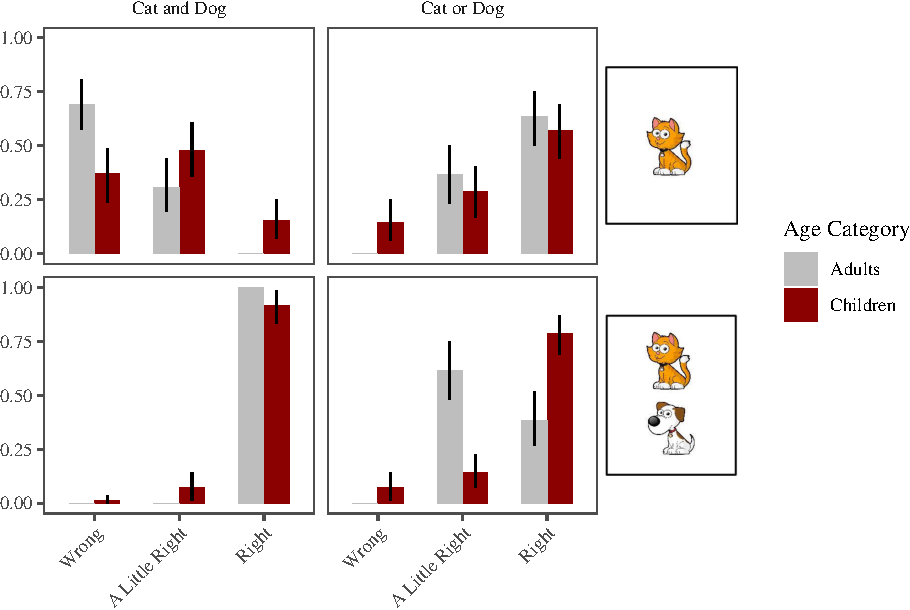
\includegraphics{Jasbi-Frank-2019_files/figure-latex/childAdultComp-1.pdf}
\caption{\label{fig:childAdultComp}Comparison of Adults' 3AFC judgments from Experiment 1 and Children's 3AFC judgments from Experiment 2.}
\end{figure}

Figure \ref{fig:childAdultComp} compares the results for children and adults' 3AFC judgments in the conjunction and disjunction trials. The major difference seems to be the cases of disjunction (e.g.~\emph{cat or dog}) when both disjuncts were true (e.g.~\textsc{cat+dog}). Children were more likely than adults to consider such utterances as \enquote{right}. To quantify possible differences between adults and children more precisely and model both our 3AFC task as well as the subject-level clustering of data, we decided to fit ordinal mixed-effects logistic models. Since ordinal and multinomial logistic models with complex random effects structures are not easily fit in standard frequentist packages, we adopted the Bayesian framework and used the R package \enquote{brms} (Bürkner, 2017).

First, we fit separate ordinal mixed-effects logistic models for adults and children. The models included the fixed effect of trial-type and maximal random-effects structures (Barr, Levy, Scheepers, \& Tily, 2013), i.e.~random intercepts and slopes for participants and items (cards).\footnote{response \textasciitilde{} trial type + (1 + trial type\textbar sid) + (1 + trial type\textbar card)} Second, we fit an ordinal mixed-effects model to the combined dataset of adults and children with the added interaction effect of \enquote{age category} (adult vs.~child), with \enquote{adults} set as the intercept.\footnote{response \textasciitilde{} trial type * age category + (1 + trial type\textbar sid) + (1 + trial type\textbar card)} Third, to understand the role of age in children's responses, we fit an ordinal mixed-effects model to children's data with \enquote{child age} as an interaction term. For all models, the response variable had three ordered levels: \enquote{wrong}, \enquote{kinda right}, and \enquote{right}\footnote{response \textasciitilde{} trial type * child age + (1 + trial type\textbar sid) + (1 + trial type\textbar card)}. The trial types \enquote{T,Con} (true conjunction), \enquote{T.in,Dis} (true-but-infelicitous disjunction), and \enquote{F,Con} (false conjunction) constituted the (dummy-coded) fixed effects of the model, with \enquote{T,Dis} (true disjunction) set as the intercept. The priors over trial types were set to \(\mathcal{N}(0,10)\). For other parameters, default weakly informative priors -- Student-t (3, 0, 10) and Cholesky LKJ Correlation (1) -- were used as endorsed in \enquote{brms} documentation. All four chains converged after 4000 samples (with a burn-in period of 2000 samples).

\begin{figure}
\centering
\includegraphics{Jasbi-Frank-2019_files/figure-latex/exp2TVJTstats-1.pdf}
\caption{\label{fig:exp2TVJTstats}Left: The mean and 95\% highest posterior density intervals for the coefficients estimated for each trial type in separate ordinal logistic regressions for adults and children. \enquote{F,Con - T,Dis} shows comparison of false conjunction and true disjunction trials; \enquote{T,Con - T,Dis} true conjunction vs.~true disjunction trials; \enquote{T.in,Dis - T,Dis} true-but-infelicitous disjunction vs.~true disjunction trials. Right: Mean and 95\% highest posterior density interval for the interaction coefficients (age category, adults as intercept) in the adult-child combined dataset. The x-axis labels stand for trial types shown in Figure 5.}
\end{figure}

We did not find any effect of children's age on their 3AFC responses. Therefore, the remainder of this section focuses on the effect of trial-types and the comparison of children and adults' responses. Figure \ref{fig:exp2TVJTstats} shows the means and the 95\% highest posterior density intervals (HPDIs) for the coefficients of these models. The left panel of Figure \ref{fig:exp2TVJTstats} shows the results from separate ordinal models for adults and children. It helps us understand how adults and children interpreted conjunction and disjunction separately. Because predictors were dummy-coded, it is possible to examine contrasts of interest by computing the difference between coefficients for pairs of conditions we wish to contrast. The x-axis shows three contrasts of interest. First, both adults and children rated false conjunction trials lower than true disjunction trials (F,Con - T,Dis) {[}children's 95\% HPDI: -4.99,
-0.16{]}. Second, both adults and children judged true conjunction trials better than true disjunction trials (T,Con - T,Dis). Nevertheless, the 95\% credible intervals for both groups contained zero. Finally, adults judged true disjunction trials slightly better than true-but-infelicitous ones while children judged true-but-infelicitous disjunction trials slightly better. However, the 95\% credible intervals for both groups contained zero. The means and credible intervals computed separately for adults and children match truth conditions of conjunction and disjunction: false conjunction trials were judged negatively and differently from true conjunction and disjunction trials.

To provide a precise estimate of the differences between adults' and children's judgments, we look at the means and the 95\% HPDIs of the interaction coefficients in the combined adult-child dataset (Figure \ref{fig:exp2TVJTstats}, Right). For false conjunction and true-but-infelicitous disjunction trials, the 95\% credible intervals do not contain zero. This suggests that children's and adults' judgments differed in these two trial types. In both trial types, children's judgments were higher than adults' judgments. This is compatible with the possible effect of two previously discussed hypotheses. First that children are more lenient than adults, and second that children's judgments are affected by how many labels match the animals on the card (Paris, 1973). However, these hypotheses are very specific to the differences between children and adults in these two trial types and do not provide a general explanation for children's responses. Finally, higher ratings in true-but-infelicitous trials are also consistent with the hypothesis that children compute exclusivity implicatures at a lower rate than adults (Barner et al., 2011; Noveck, 2001; Papafragou \& Musolino, 2003).

\hypertarget{open-ended-verbal-feedback}{%
\subsubsection{Open-ended Verbal Feedback}\label{open-ended-verbal-feedback}}

We also categorized and annotated children's spontaneous and free-form verbal feedback to the puppet's guesses before they made their forced-choice judgments. Table \ref{tab:feedbackCat} summarizes the definitions and examples for each category and Figure \ref{fig:exp2feedbackPlot} shows the results. We should point out that each trial type had a similar number of \enquote{None} cases. Some children remained silent throughout the experiment and only provided rewards to the puppet. In Experiment 3, we explicitly asked children to provide feedback and therefore, had no \enquote{None} response category. In the discussion and analysis here we will not comment further on the \enquote{None} category but focus on the other three categories.

\begin{figure}
\centering
\includegraphics{Jasbi-Frank-2019_files/figure-latex/exp2feedbackPlot-1.pdf}
\caption{\label{fig:exp2feedbackPlot}Children's open-ended vebal feedback in Experiment 2 classified as \enquote{judgments} (yes/no), \enquote{descriptions} (e.g.~cat, dog, cat and dog), and \enquote{corrections} (e.g.~just a cat, only a cat, \enquote{cat AND dog}, Both!).}
\end{figure}

Starting with the leftmost column of Figure \ref{fig:exp2feedbackPlot}), in false simple trials the guessed animal was not on the card (e.g.~\emph{elephant}) and children either provided judgments like \enquote{No!} or descriptions like \enquote{cat} or \enquote{cat and dog}. Moving to the second column, in true simple trials the guessed animal (e.g.~\emph{cat}) was the only animal on the card and most children provided positive judgments like \enquote{Yes}. In true-but-incomplete trials, the animal guessed (e.g.~\emph{cat}) was only one of the two animals on the card (e.g.~\textsc{cat+dog}) and children provided a description of the the card, for example \enquote{cat and dog}.

In false conjunction trials, only one of the animal was on the card when two were guessed (e.g.~\emph{cat and dog}) In such trials, children provided a high number of corrections and descriptions. The category \enquote{corrections} here means that children used the focus particles \emph{just} and \emph{only} as in \enquote{just a cat} or \enquote{only a cat}. In true conjunction trials, both animals were on the card and children predominantly provided positive judgments like \enquote{Yes!}. With true disjunction trials, only one of the guessed animals was on the card and most children simply provided a description of what was on the card (e.g.~\enquote{cat}). However, in true-but-infelicitous disjunction trials, both animals were on the card yet children provided corrections like \enquote{Both!} or emphasizing \emph{and} as in \enquote{cat AND dog!}.

\begin{figure}
\centering
\includegraphics{Jasbi-Frank-2019_files/figure-latex/exp2FeedbackStats-1.pdf}
\caption{\label{fig:exp2FeedbackStats}The mean and 95\% highest posterior density interval of the coefficients of interest in experiment 2's mixed-effects multinomial logistic model on children's feedback. The category \enquote{correction} was set as the reference category and \enquote{Infelicitous Disjunction Trials} were set as the intercept of the model.}
\end{figure}

To quantify and compare the distribution of children's spontaneous feedback in different trial-types, we used a Bayesian mixed-effects multinomial regression model with the fixed effect of trial-type as well as random intercepts and slopes for participants and items (cards).\footnote{feedback \textasciitilde{} trial type + (1 + trial type\textbar sid) + (1 + trial type\textbar card)} The dependent measure was children's feedback categories of judgment, description, and correction, with correction set as the reference category. The trial types \enquote{T,Dis}, \enquote{F,Con}, and \enquote{T,Con} constituted the (dummy-coded) fixed effects of the model with \enquote{T.in,Dis} set as the intercept. To test the effect of children's age on their corrective feedback, we used a similar model but added the interaction term \enquote{child age}. Priors and convergence information were identical to those reported for our previous models.

We did not find any effect of children's age on their verbal feedback. Therefore, the remainder of this section focuses on the model without the effect of age. Figure \ref{fig:exp2FeedbackStats} shows the means and 95\% credible intervals of the multinomial model coefficients, with the x-axis separating trial types. Starting from the left, the credible intervals for judgments and descriptions over corrections for the \enquote{F,Con} trial-type included zero. This suggests that the feedback distribution was similar in false conjunction trials and true-but-infelicitous disjunction trials. Both trial types received a relatively high number of corrections. With \enquote{T,Con} trials, the credible interval for descriptions over corrections covers zero while that of judgments over corrections stays above zero. This suggests that with true conjunctions children provided more affirmative judgments like \enquote{yes} than corrections. Finally with \enquote{T,Dis} trials, even though children provided more descriptions, the credible intervals for judgments and descriptions over corrections included zero. As we will see in the next experiment where we register and replicate children's verbal feedback, children do provide more descriptions than corrections in true disjunction trials.

\hypertarget{discussion-1}{%
\subsection{Discussion}\label{discussion-1}}

In Experiment 2, we used a 3AFC judgment task to test children's comprehension of logical connectives \emph{and} and \emph{or}. We compared these results to those found in the 3AFC judgment task of Experiment 1 with adults. The general comparison showed that adults and children had similar patterns of judgments with respect to the truth conditional semantics of the connectives. Both groups had negative judgments for false conjunction statements and positive judgments for true conjunction and disjunction trials. Furthermore, we did not find any effect of children's age on their forced-choice judgments. This suggests that 3-to-5-year-old children understood the semantics of linguistic conjunction and disjunction in an adult-like manner. However, the results also showed that children's judgments differed from adults in two ways. First, children were more likely to consider a conjunction guess \enquote{kinda right} (and reward the puppet) when it was false. Second, children were more likely to consider a disjunction guess \enquote{right} (and reward the puppet) when the guess was infelicitous and potentially carried an exclusivity implicature. This second difference is consistent with the hypothesis that children compute implicatures at a lower rate than adults. However, our analysis of children's spontaneous verbal feedback provided evidence that children are sensitive to this infelicity and exclusivity implicature.

Children often volunteered open-ended verbal feedback to the puppet's guesses before they made their forced-choice judgments. Our analysis of this feedback showed that children's feedback was sensitive to the semantics and pragmatics of the experimental utterances. Children provided more instances of \enquote{correction} when the utterance was false or carried a defeasible false implicature (exhaustive or scalar). As expected from an adult-like understanding of connectives, children corrected the puppet most often when a conjunction was false (i.e.~only one proposition was true), or when a disjunction was infelicitous (i.e.~both propositions were true) and could carry a false exclusivity implicature. We did not find evidence for any age effect on children's verbal feedback either. The forced choice judgments suggest that children in this age range understood the truth conditions of conjunction and disjunction. Children's spontaneous verbal feedback showed that they might be sensitive to the pragmatic infelicity of a disjunction when both disjuncts were true. Children often explicitly mentioned \emph{and} as the connective that should have been used in such contexts instead of \emph{or}. In the next Experiment, we follow up on these finding and replicate the results of Experiment 2 in a two-alternative forced-choice task.

\hypertarget{study3}{%
\section{Experiment 3: Children's 2AFC judgments and open-ended feedback}\label{study3}}

This study used the same paradigm as Experiment 2 but measured children's judgments using a binary forced choice task. Similar to Experiment 2, children's open-ended feedback was also analyzed. The main hypothesis was that preschool children provide corrective feedback if the disjunction is true but infelicitous. However, they do not consider this infelicity to be grave enough to render the guess \enquote{wrong} in a 2AFC judgment task. The main hypothesis along with relevant analyses and predictions were preregistered in an \enquote{As Predicted} format\footnote{The As Predicted PDF document is accessible at \url{https://aspredicted.org/x9ez2.pdf}. We deviated from our primary analysis because the availability of software for fitting Bayesian multinomial regression models allowed us to fit a similar but more appropriate model that included a broader variety of response types. We did not carry out the secondary analyses that we thought we might. The main reason was that they were not carried out in Experiment 2, and that they were not related to the main hypothesis being tested.}.

\hypertarget{methods-2}{%
\subsection{Methods}\label{methods-2}}

\hypertarget{participants-2}{%
\subsubsection{Participants}\label{participants-2}}

We recruited 50 English speaking children from the Bing Nursery School at Stanford University. Children were between 3;6 and 5;9 years old (Mean = 4;7). Parents of children had provided written informed consent for this experiment.

\hypertarget{materials-1}{%
\subsubsection{Materials}\label{materials-1}}

Experiment 3 was similar to Experiment 2 but differed in how children provided their judgments. Based on the findings in Experiment 2, we focused on verbal feedback, instead of forced-choice responses. We used two different ways of measuring children's judgments. First, we encouraged children to provide verbal feedback to the puppet. They were asked to say \enquote{yes} when the puppet was right and \enquote{no} when he was not right. Importantly, they were also asked to help him say it better. In each trial, after children were done with this initial open-ended feedback, we asked the classic truth value judgment forced choice question: \enquote{Was Jazzy (the puppet) right?}. This question elicited a 2AFC response for each trial independent of children's earlier open-ended response. These two measures allowed us to compare open-ended and binary forced-choice judgments in the same paradigm and for the same trials.

\hypertarget{procedure-2}{%
\subsubsection{Procedure}\label{procedure-2}}

The setup and procedure were similar to Experiment 2, except there were no rewards. As in previous studies, participants sat through three phases: introduction, instruction, and test. The introduction phase made sure children knew the names of the animals on the cards. In the instruction phase, they received four training trials, as shown in Table \ref{tab:instructionStudy3} in the Appendix section.

As in Experiment 2, the experimenter put a sleeping mask over the puppet's eyes and explained that Jazzy (the puppet) was going to guess what animal was on the cards. He then picked the first card and asked the puppet: \enquote{What do you think is on this card?} The puppet replied with \enquote{There is a dog}. The experimenter showed the cat-card to the child and said: when Jazzy is \enquote{not right}, tell him \enquote{no}. He then asked the child to say \enquote{no} to the puppet. The second trial followed the same pattern except that the puppet guessed \enquote{right} and the experimenter invited the child to say \enquote{yes} to the puppet. There were two more instruction trials before the test phase began. The test phase contained 16 randomized trials, half of which contained guesses with the words \emph{and} and \emph{or}\footnote{The randomization code as well as the details of the methods are available on this paper's online repository.}.

\hypertarget{results-2}{%
\subsection{Results}\label{results-2}}

We first look at the results of the 2AFC judgement task for each trial type and compare them to those of the adults' in Experiment 1. Then we analyze children's open-ended verbal feedback and compare them to the forced choice responses obtained in the same trial types. We should emphasize that similar to Experiment 2, the open-ended feedback was produced before the forced-choice responses and cannot count as verbal justifications for such responses. For the 2AFC judgments we excluded 26 trials (out of total 800) where children either did not provide a Yes/No response or provided both (i.e.~\enquote{Yes and No}). The exclusions were almost equally distributed among different types of guesses and cards. In the analysis of children's open-ended feedback, we excluded 8 trials (out of total 800) where children either did not provide any feedback or their feedback could not be categorized into the existing categories.

\hypertarget{two-alternative-forced-choice-judgments}{%
\subsubsection{Two-Alternative Forced Choice Judgments}\label{two-alternative-forced-choice-judgments}}

\begin{figure}
\centering
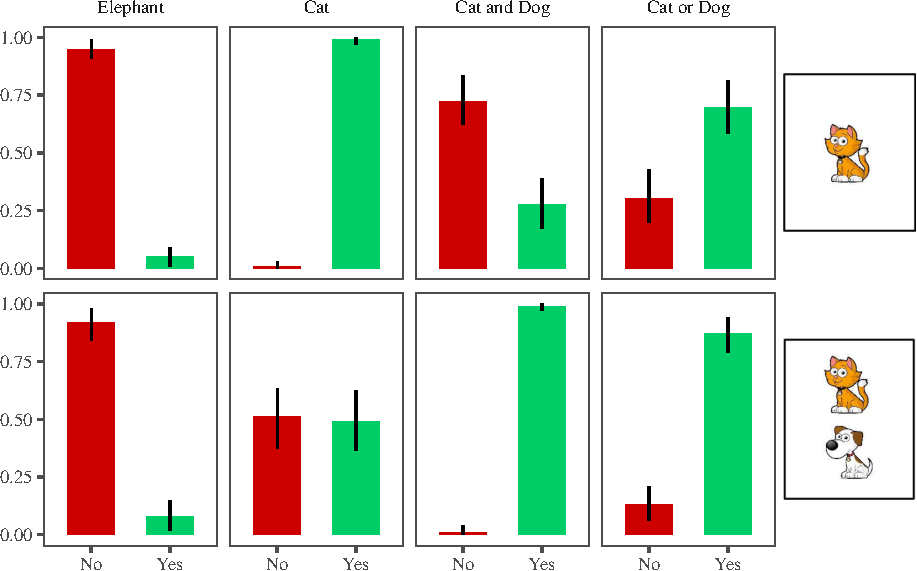
\includegraphics{Jasbi-Frank-2019_files/figure-latex/Study3tvjtPlot-1.pdf}
\caption{\label{fig:Study3tvjtPlot}Children's two-alternative forced-choice judgments in Experiment 3.}
\end{figure}

Figure \ref{fig:Study3tvjtPlot} shows children's 2AFC judgments. Starting with the leftmost column and false simple trial types, the guessed animal (e.g.~\emph{elephant}) was not on the card and children considered the guess \enquote{wrong}. Moving to the next column and true simple trials, the guessed animal (e.g.~\emph{cat}) was the only animal on the card and children considered the guess \enquote{right}. In true-but-incomplete trials only one of the animals was guessed and children's judgments were equally split between \enquote{wrong} and \enquote{right}. This is in contrast to adults who unanimously considered such guesses as \enquote{right} in their 2AFC judgments (Figure \ref{fig:binaryAdultsPlot}). There are two possible explanations for this difference. First, some children may interpret a simple guess like \enquote{there is a cat} exhaustively as \enquote{there is \textbf{only} a cat}. Second, some children may consider leaving out an animal as a grave violation even though they do not interpret the guess as there is \textbf{only one} animal on the card. The first explanation is unexpected for a theory of acquisition that assumes children are overall more logical or literal interpreters than adults (Noveck, 2001).

In false conjunction trials, only one of the two guessed animals was on the card and most children considered the guess \enquote{wrong}. These binary judgments are similar to those of adults', but different in extent: adults were more consistent and unanimous in rejecting such guesses. In true conjunction trials, children unanimously judged the guess \enquote{right}, similar to adults. In true disjunction trials, the card had only one of the guessed animals and most children considered the guess \enquote{right}. This is again similar to adults but differs from them in extent: adults more consistently and unanimously judged such guesses as \enquote{right}. Finally, with true-but-infelicitous disjunction trials, children considered the guess \enquote{right}.

\begin{figure}
\centering
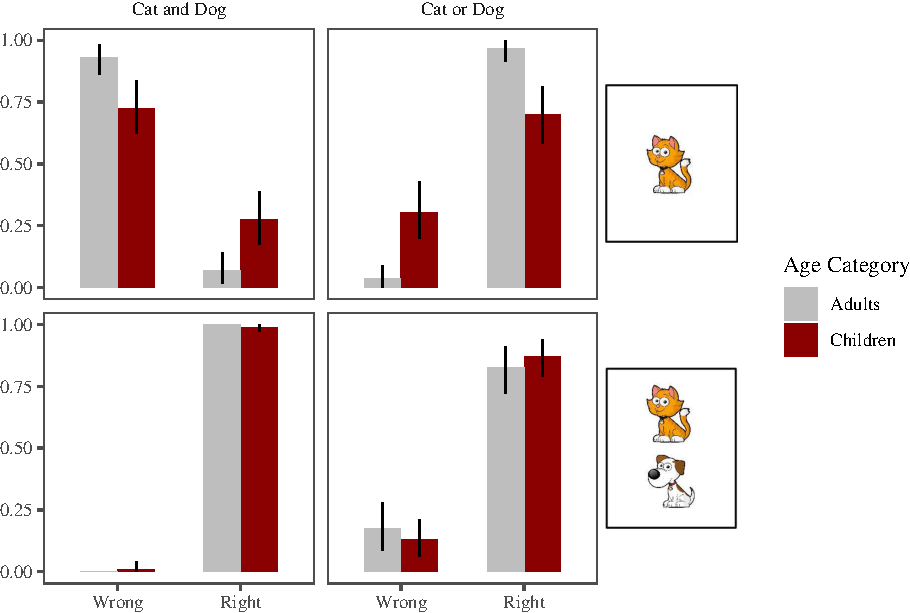
\includegraphics{Jasbi-Frank-2019_files/figure-latex/BinaryPlotComp-1.pdf}
\caption{\label{fig:BinaryPlotComp}The comparison of 2AFC judgment tasks for conjunction and disjunction trials in adults (Experiment 1) and children (Experiment 3).}
\end{figure}

Figure \ref{fig:BinaryPlotComp} provides a side-by-side comparison of adults' and children's 2AFC judgments for conjunction and disjunction trials. The judgments are similar but differ somewhat in trial types where there is only one animal on the card. To quantify trial-type differences in adults and children, we fit separate Bayesian mixed-effects binomial logistic regressions for each group, with \enquote{trial-type} as a predictor. Similarly, to capture differences between adults and children, we fit a model to the combined dataset of adults and children and added age category (adult vs.~child) as an interaction term. Finally, to check the effect of age on children's forced-choice responses, we fit a similar model to children's data with \enquote{child age} as an interaction term. These models mirror what we did in our analysis of Experiment 2 data. As in Experiment 2, the models included the fixed dummy coded effect of trial-type (Levels: \enquote{T,Dis} (reference) - \enquote{T,Con} - \enquote{F,Con} - \enquote{T.in,Dis}). The models also included random intercepts and slopes for participants and items. Details of priors and convergence were similar to the models in Experiment 2 as well.

\begin{figure}
\centering
\includegraphics{Jasbi-Frank-2019_files/figure-latex/exp3TVJTstats-1.pdf}
\caption{\label{fig:exp3TVJTstats}Left: The means and 95\% highest posterior density intervals for parameter values estimated in separate ordinal logistic regressions for adults and children. \enquote{F,Con - T,Dis} shows the comparison of false conjunction and true disjunction trials; \enquote{T,Con - T,Dis} true conjunction vs.~true disjunction trials; \enquote{T.in,Dis - T,Dis} true but infelicitous disjunction vs.~true disjunction trials. Right: The means and 95\% highest posterior density intervals for the interactive effect of age category (child vs.~adult, adult intercept) on 2AFC judgments. The x-axis labels represent false conjunction, true conjunction, true disjunction, and true but infelicitous disjunction trials.}
\end{figure}

Similar to Experiment 2, we did not find any age effect in children's forced choice judgments. Therefore, the rest of this section focuses on the effects of trial types and comparison of children's responses with those of adults. The left panel of Figure \ref{fig:exp3TVJTstats} shows the means and 95\% HPDIs for three contrasts of interest shown on the x-axis, estimated from separate binomial models for adults and children. First, for both adults and children, the 95\% credible intervals for \enquote{F,Con - T,Dis} do not contain zero. This suggests that for both groups, judgments of false conjunction trials were lower and different than true disjunction trials. Second, 95\% credible intervals for \enquote{T,Con - T,Dis} estimated for adults and children contains zero. Therefore, adults and children had similar judgments for true conjunction and true disjunction trials. Third, the 95\% credible intervals for \enquote{T.in,Dis - T,Dis} contains zero as well, suggesting that children and adults judged true-but-infelicitous disjunction trials similar to the true disjunction trials. Overall, the separate binomial models show that judgment patterns match the truth conditional semantics of conjunction and disjunction. False conjunction trials were judged negatively and differently from true conjunction and disjunction trials.

To estimate the extent to which adults' and children's judgments differed from each other, we looked at the means and the 95\% credible intervals of the interaction coefficients computed in the combined binomial model (Figure \ref{fig:exp3TVJTstats}, Right). Based on the 95\% credible intervals, we can infer that judgments of adults and children differed in three ways. First, children judged false conjunction trials slightly more positively than adults (F,Con). Second, they judged true disjunction trials slightly more negatively than adults (T,Dis). Notice that these two differences between children and adults are compatible with a small effect of label-matching (Paris, 1973), given that for both of these trials there is a mismatch between the mentioned labels and the animal on the card. However, non-adult-like pragmatic enrichment cannot explain this pattern (Singh2016, Tieu et al., 2017). Pragmatic enrichment predicts that children would rate a true disjunction more negatively than adults, but does not predict more positive judgments for false conjunction trials. However, the label-matching account predicts both these outcomes, because it posits that in both cases, the partial match between animal labels and animal pictures affects children's judgments. Nevertheless, this effect is small and label-matching cannot provide a general explanation for children's responses given that with the same labels (e.g \emph{cat}, \emph{dog}) and picture (e.g.~\textsc{cat}) the use of the connective (\emph{or} vs.~\emph{and}) creates significant differences in judgments. Finally in the third difference, children judged true but infelicitous disjunction trials more positively than adults did. This is consistent with the hypothesis that children compute exclusivity implicatures at a lower rate than adults. However, as we will see in the next section, children's spontaneous verbal feedback paints a more nuanced picture regarding exclusivity implicatures in children.

\hypertarget{open-ended-verbal-feedback-1}{%
\subsubsection{Open-ended Verbal Feedback}\label{open-ended-verbal-feedback-1}}

\begin{figure}
\centering
\includegraphics{Jasbi-Frank-2019_files/figure-latex/exp3feedbackPlot-1.pdf}
\caption{\label{fig:exp3feedbackPlot}Children's open-ended vebal feedback in Experiment 3 classified as \enquote{judgments} (yes/no), \enquote{descriptions} (e.g.~cat, dog, cat and dog), and \enquote{corrections} (e.g.~just a cat, only a cat, \enquote{cat AND dog}, Both!)..}
\end{figure}

Figure \ref{fig:exp3feedbackPlot} shows the distribution of children's feedback to the puppet in Experiment 3 (see Table \ref{tab:feedbackCat} for the definitions and examples of feedback categories). Similar to Experiment 2, children's feedback showed four main patterns. First in false simple trial types when the puppet guessed an animal not on the card (e.g.~\emph{elephant}), there was a split pattern between negative judgments like \enquote{No!} and descriptions like \enquote{Cat!}. Second, almost all children responded with positive judgments like \enquote{Yes!} in true simple and true conjunction trial types. These are the trials where the puppet's guess correctly and optimally matched what was on the card. Third, in true disjunction trials where the puppet used a disjunction (e.g.~\emph{cat or dog}) with only one of the animals on the card, almost all children named the animal on the card (e.g.~\enquote{cat!}). Fourth and most importantly, children provided corrections in trials where a guess was either false or infelicitous (could carry a defeasible false implicature). These included three trial types. First, true but incomplete simple trials in which two animals were on the card (e.g.~\textsc{cat+dog}) but the puppet only guessed one (e.g.~\emph{cat}). Such trials can carry a defeasible false exhaustivity implicature. Second, false conjunction trials in which the puppet guessed two animals (e.g.~\emph{cat and dog}) but only one of them was on the card (e.g.~\textsc{cat}). Third, true but infelicitous disjunction trials in which two animals were on the card (e.g.~\textsc{cat+dog}), and the puppet guessed both but used a disjunction (e.g.~\emph{cat or dog}). Such trials can carry a defeasible false exclusivity implicature.

\begin{figure}
\centering
\includegraphics{Jasbi-Frank-2019_files/figure-latex/exp3FeedbackStats-1.pdf}
\caption{\label{fig:exp3FeedbackStats}The means and 95\% highest posterior density intervals of the coefficients of interest in experiment 3's mixed-effects multinomial logistic model on children's feedback. The category \enquote{correction} was set as the reference category and \enquote{Infelicitous Disjunction Trials} were set as the intercept of the model.}
\end{figure}

To quantify and compare the distribution of children's feedback in trial types with connectives, we used a Bayesian mixed-effects multinomial regression model with the fixed effect of trial-type as well as random intercepts and slopes for participants and items (cards). Similar to our analysis in Experiment 2, the dependent measure was children's feedback categories of judgment, description, and correction, with correction set as the reference category. The trial-types \enquote{F,Con}, \enquote{T,Con}, \enquote{T,Dis} constituted the (dummy-coded) fixed effects of the model with \enquote{T.in,Dis} set as the intercept. Priors and convergence information were identical to those reported for our previous models.

Figure \ref{fig:exp3FeedbackStats} shows the means and 95\% credible intervals of the multinomial model coefficients. These results replicate the findings on children's feedback reported in Experiment 2. Starting from the left, the credible intervals for judgments over corrections as well as descriptions over corrections for false conjunction trials (F,Con) include zero. This suggests that the feedback distribution was similar in false conjunction and true-but-infelicitous disjunction trials. In true disjunction trials (T,Dis), the credible interval for judgments over corrections includes zero but not that of descriptions. Therefore, children provided more descriptions than corrections in true disjunction trials (T,Dis). Finally with true conjunction trials (T,Con), the credible interval for descriptions over corrections includes zero, but not judgments over corrections. This suggests that with true conjunctions, children provided more affirmative judgments like \enquote{yes} than corrections. Overall, the results confirm the findings reported in Experiment 2: children were more likely to provide corrections in trial-types that were either false or could carry a false defeasible implicature (exhaustive or scalar).

\begin{figure}
\centering
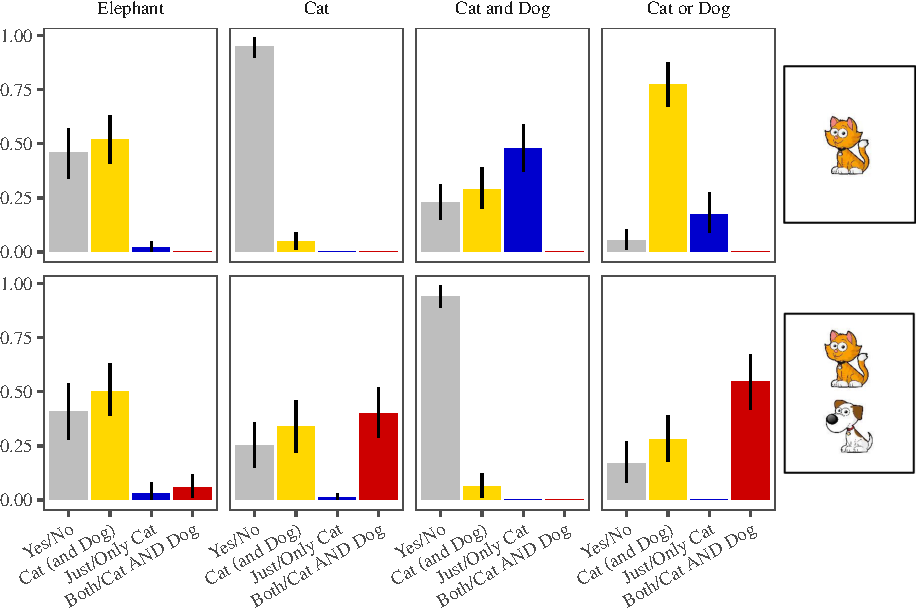
\includegraphics{Jasbi-Frank-2019_files/figure-latex/correctivePlot-1.pdf}
\caption{\label{fig:correctivePlot}Children's open-ended feedback in different trial types of Experiment 3.}
\end{figure}

To better appreciate the pattern of spontaneous corrections provided by children, Figure \ref{fig:correctivePlot} breaks down corrections into two sub-categories: those using exclusive focus words such as \emph{only} and \emph{just} (blue) and those using inclusive focus elements such as \emph{both} and emphasizing \emph{AND}. Our goal here is to focus on the trial types with corrective feedback (blue and red). The type of corrective feedback children provided in these trial types matched the type of mistakes made in the guesses. With conjunction guesses (e.g.~\emph{cat and a dog}) when there was only one animal on the card (e.g.~\textsc{cat}), children provided exclusive corrections such as \enquote{just a cat} or \enquote{only a cat!}, suggesting that the other animal in the guess (e.g.~\emph{dog}) should have been excluded. When two animals were on the card (e.g.~\textsc{cat+dog}) and the puppet used a disjunctive guess (e.g.~\emph{cat or dog}), or a simple guess (e.g.~\emph{cat}), children provided inclusive feedback such as \enquote{cat AND dog} or \enquote{both}, suggesting that another animal should have been included. This is particularly notable in the case of disjunction since both animals were mentioned, but children still emphasized that the connective \emph{and} should have been used, or that \emph{both} animals mentioned were actually on the card. Such corrective comments hint at a good understanding of differences between the meaning and usage of the connectives.

\hypertarget{discussion-2}{%
\subsection{Discussion}\label{discussion-2}}

Experiment 3 measured children's comprehension of logical connectives in two ways: First, with analyzing their open-ended feedback and second, with a two-alternative forced choice task. The 2AFC responses followed the predicted pattern: a false conjunction was judged \enquote{wrong} and a true conjunction \enquote{right}. Disjunction guesses were judged right whether they were true or true-but-infelicitous. Children's open-ended feedback in Experiment 3 replicated the findings of Experiment 2. Children's feedback was sensitive to the pragmatics of connective use. They provided more corrective feedback when the utterance was false or could carry a false defeasible implicature. Furthermore, the corrective feedback was tailored to the puppet's mistake. If the puppet used a conjunction when there was only one animal on the card, children pointed out that the other animal should have been excluded from the guess. They used the exclusive adverbials \emph{just} and \emph{only} in their feedback. If the puppet used a disjunction when both animals were on the card, children stressed \emph{and} or \emph{both}, implying that both animals should have been included. Taking both measures into account, we conclude the following: children's 2AFC judgments suggest that they understand the basic truth-conditional semantics of \emph{or} in simple existential sentences as inclusive disjunction. Specifically, when both disjuncts are true, they do not consider an infelicitous disjunction \enquote{wrong}. In addition, children's spontaneous verbal feedback suggests that they consider a conjunction to be a more appropriate utterance in such cases.

\hypertarget{general-discussion}{%
\section{General Discussion}\label{general-discussion}}

Almost a century has passed since Alfred Tarski observed that disjunction gives rise to complex implications with important psychological effects. To Tarski, these implications appeared unsystematic and informal. Paul Grice, however, considered them a natural consequence of human rational and social interaction. Following Grice's insights, research in formal semantics and pragmatics has discovered a great deal of systematicity in how we interpret linguistic disjunction. This theoretical progress has in turn led to experimentally testable predictions about the comprehension of disjunction and how it develops in children. Developmental studies in the past two decades have argued that preschool children understand the basic semantics of disjunction. Yet the pragmatic inferences they derive from the use of disjunction has been argued to differ from those derived by adults in two ways. First, due to non-adult-like reasoning, children are more likely to interpret \emph{or} as \emph{and} (conjunctive interpretations; Singh et al., 2016; Tieu et al., 2017); Second, children are more likely to consider a disjunction as inclusive (lack of exclusivity implicatures; Chierchia et al., 2001, 2004; Crain, 2008).

Using three different types of measurement, this study investigated adults' and children's comprehension of linguistic disjunction in simple existential sentences. The results of our experiments confirmed previous findings that adults and preschool children understand the truth-conditional semantics of \emph{or} as inclusive disjunction (Chierchia et al., 1998, 2004; Crain, 2012). With respect to children's pragmatic reasoning, however, our experiments suggested that children's pragmatic reasoning may be more adult-like than previously argued. First, our experiments did not provide evidence for conjunctive interpretations of disjunction, confirming previous studies that have argued such findings may be due to task characteristics and demands (Braine \& Rumain, 1981; Paris, 1973; Skordos et al., 2020). Second and with respect to exclusivity implicatures, we found conflicting results based on the type of measurement used. Specifically, our three-alternative forced-choice task suggested that adults but not children, show sensitivity to the exclusivity implicature of disjunction. However, the quantitative analysis of children's spontaneous verbal reactions showed that children were also sensitive to such exclusivity implicatures, or at least that \emph{and} is a better connective in such cases. More concretely, children explicitly mentioned \emph{and} as the alternative that should have been used in contexts where both disjuncts were true and \emph{or} was used instead.

The results reported here have two main implications for developmental semantics and pragmatics. First, children's conjunctive interpretations of disjunction in some of the previous studies have been attributed to a particular theory of pragmatic implicatures (Fox, 2007) and a developmental account in which children differ from adults with respect to the set of alternatives they generate while computing such implicatures (Singh et al., 2016; Tieu et al., 2017). However, as explained in our literature review, there is substantial evidence that conjunctive interpretations, even when robustly observed, are likely due to task demands and application of non-linguistic strategies (Braine \& Rumain, 1981; Neimark \& Slotnick, 1970; Paris, 1973; Skordos et al., 2020). Therefore, in order to show instances of pragmatically enriched conjunctive readings in preschool children, it is crucial to first rule out conjunctive interpretations due to task demands and application of non-linguistic strategies. Advocates of pragmatically enriched conjunctive readings could achieve this goal by including trials in which the disjunction word (e.g.~\emph{or}) is replaced by a nonsense word. If it is truly the disjunction word that children enrich pragmatically via non-adult-like alternatives, then trials with the disjunction word should elicit higher conjunctive interpretations than control trials with the nonsense word.

Second, there are three major proposals to account for children's observed lower rate of scalar implicatures in experimental tasks (Noveck, 2001; Papafragou \& Musolino, 2003). The first proposal focuses on processing difficulty, suggesting that implicature computations are cognitively taxing and children lack the appropriate processing resources (Pouscoulous, Noveck, Politzer, \& Bastide, 2007; Reinhart, 2004). The second proposal is that children have not learned the scale (e.g.~\textless{}\emph{or}, \emph{and}\textgreater), which allows for derivation of adult-like scalar implicatures (Barner et al., 2011; Horowitz, Schneider, \& Frank, 2017). According to this proposal, children either lack the meaning for \emph{or}, lack the meaning for \emph{and}, or have not assigned \emph{and} as the stronger alternative to \emph{or}. Finally, the third proposal is that children are more tolerant of pragmatic infelicities than adults (Katsos \& Bishop, 2011). When a speaker uses a linguistic form (e.g.~a disjunction) that is true but not felicitous, children tolerate it and consider it \enquote{right} but adults do not.

The experimental results presented here do not fit the predictions of these previous accounts and show more nuance regarding the development of implicatures. We found that children were more likely than adults to judge a disjunction \enquote{right} when both propositions were true. This phenomenon is often referred to as \enquote{lack of scalar implicatures} in children. Yet, we also found that children were more likely than adults to judge a simple guess (e.g.~cat) as \enquote{wrong} when there were two animals (e.g.~\textsc{cat+dog}). In other words, children were more likely to interpret a simple guess (e.g.~\enquote{there is a cat}) exhaustively (e.g.~\enquote{there is \emph{only} a cat}). Let's call this pattern \enquote{surplus of exhaustivity implicatures} in children. Neither the processing account nor the tolerance account predict \enquote{lack of scalar (exclusivity) implicatures} as well as \enquote{surplus of exhaustivity implicatures} in preschool children. Whether children struggle with processing pragmatic inferences, or they are more tolerant of pragmatic violations, we should observe the lack of implicatures across the board.

Non-adult-like knowledge of the scale \textless{}\emph{or}, \emph{and}\textgreater{} does not explain the results presented here either. Our experiments showed that preschool children differentiated \emph{or} from \emph{and}, interpreting each similar to adults (modulo exclusivity). Therefore, it is unlikely that children did not know the meaning of the weak member of the scale (i.e.~\emph{or}) or the strong member of the scale (i.e.~\emph{and}). Moreover with true-but-infelicitous disjunction trials, many children who judged the disjunction as \enquote{right} also informed the puppet in their verbal feedback that \emph{and} should have been used instead. Mentioning \emph{and} as the more felicitous alternative to \emph{or} undermines the argument that children are not aware of \emph{and} as the \enquote{scale-mate} to \emph{or}. Taken together, the results of children's forced-choice judgments and their verbal feedback suggest many children understood that the puppet should have used \emph{and} instead of \emph{or}, yet they did not consider this infelicity grave enough to render the guess \enquote{wrong} or even \enquote{kinda right}.

Instead, we suggest that these experimental results are compatible with two alternative hypotheses. First, it is possible that even though children know the meaning of the connectives, and know that \emph{and} is the stronger alternative to \emph{or} (e.g.~they know the scale), they still do not derive an exclusivity implicature. In other words, children know that when both propositions are true, the speaker should have used \emph{and} instead of \emph{or}, but they do not infer that the speaker believed the conjunction to be false. At the same time, when both propositions are true (e.g.~\textsc{cat+dog}) and only one is asserted (e.g.~\emph{cat}), children know that a conjunction (e.g.~\emph{cat and dog}) is the stronger alternative, and they derive an exhaustivity implicature; in fact more frequently than adults according to our binary task.\footnote{We would like to thank Roman Feiman for encouraging us to develop this alternative hypothesis.} What can explain children's success with exhaustive implicatures but failure with scalar ones even though they show knowledge of the scale? One possibility is that children are uncertain about the \enquote{mutual knowledge of the scale}: that both them and the speaker know that \emph{and} is the stronger alternative to \emph{or}. Under this hypothesis, children would not punish the speaker by choosing \enquote{wrong} or \enquote{kinda right} because they are not sure whether the speaker has the knowledge that \emph{and} is the stronger alternative to \emph{or}. However, they know the scale themselves and they are happy to offer it verbally in their reactions or feedback. On the other hand, they might have an easier time assuming that ad-hoc nominal scales \textless{}\emph{cat}, \emph{cat and dog}\textgreater{} are mutually known given that such scales do not require knowledge of subtle function words. The common use of puppets in developmental studies like ours may have contributed to this phenomenon, given that children may have more uncertainty regarding linguistic abilities of puppets.

The second hypothesis is that children and adults differ in how they use the \enquote{right}-\enquote{wrong} response scale and what types of linguistic violations they consider \enquote{wrong}. Even though the truth value judgment task commonly uses the \enquote{wrong}-\enquote{right} scale to measure semantic and pragmatic knowledge, it is not clear how different theoretical constructs such as entailment, presupposition, implicature, or infelicity link to this scale and affect our conclusions. More importantly, it is not clear whether this linking is the same for adults and children. Children may differ from adults with respect to which linguistic violations would make an utterance \enquote{wrong} or punishable. They might consider a violation in connective use (\emph{or} vs.~\emph{and}) much less severe than an incomplete assertion (\emph{cat} vs.~\emph{cat and dog}). Given that the notions \enquote{wrong} and \enquote{right} are subject to development with respect to other types of social behavior, it might not be surprising to see the same with respect to linguistic behavior. This issue is further compounded when we consider implicature not as a binary phenomenon (generated vs.~not), but rather as an inference with degrees of strength and certainty (Frank \& Goodman, 2012; Goodman \& Frank, 2016). Future research should systematically explore different linking hypotheses between theoretical semantic/pragmatic constructs and experimental measurements, establishing which types of measurements are most suitable for particular constructs, especially in adults vs.~children.

Since Tarski's original observations on disjunction, research in semantics and pragmatics has shown that the variety of implications Tarski observed are in fact distinct types of meaning observed in many aspects of language and connected to distinct processes that generate them. Therefore, while the inclusive implication is hypothesized to be part of the semantics of linguistic disjunction, exclusivity and ignorance are analyzed as distinct pragmatic inferences generated separately. This theoretical insight has in turn lead developmental researchers to seek distinct developmental mechanisms for each type of meaning. The results of the studies reported here suggest that as more and more varieties of meaning become subject to experimental studies, we may also need to pay closer attention to which types of measurement may be more suitable to capture the specific aspect of meaning under investigation.

\hypertarget{data-statement}{%
\section{Data Statement}\label{data-statement}}

All materials, data, and code for this article are available in the Open Science Framework Repository \url{https://osf.io/jhw8s}

\hypertarget{declaration-of-competing-interest}{%
\section{Declaration of Competing Interest}\label{declaration-of-competing-interest}}

The authors declare that there are no conflict of interest.

\hypertarget{credit-authorship-contribution-statement}{%
\section{CRediT authorship contribution statement}\label{credit-authorship-contribution-statement}}

Masoud Jasbi: Conceptualization, Methodology, Formal analysis, Data curation, Visualization, Writing - original draft, Writing - review \& editing. Michael C. Frank: Conceptualization, Methodology, Formal analysis, Writing - review \& editing, Supervision, Funding acquisition.

\hypertarget{acknowledgements}{%
\section{Acknowledgements}\label{acknowledgements}}

We would like to thank Eve V. Clark, Christopher Potts, Ellen Markman, and Susan Carey for their generous help and advice on this project. We would also like to thank the staff and children at Stanford's Bing Nursery School. This work was supported by NSF \#1456077 and the Stanford University fellowship to Masoud Jasbi.
\# Appendix

\begin{figure}

{\centering 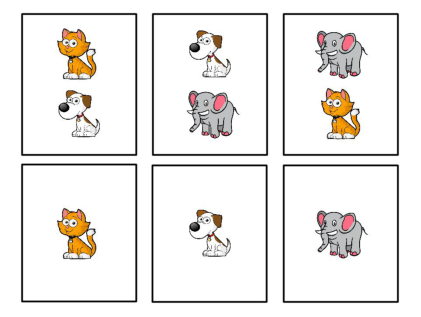
\includegraphics{Jasbi-Frank-2019_files/figure-latex/stimuli-1} 

}

\caption{Cards used in the connective guessing game, sample scenario for adults in Experiment 1, and the puppet in children's experiments with the sleeping mask on and off.}\label{fig:stimuli}
\end{figure}

\begin{longtable}[]{@{}lll@{}}
\caption{\label{tab:instruction} Instruction Trials.}\tabularnewline
\toprule
Card & Guess & Reward\tabularnewline
\midrule
\endfirsthead
\toprule
Card & Guess & Reward\tabularnewline
\midrule
\endhead
CAT & There is a dog! & Circle\tabularnewline
ELEPHANT & There is an elephant! & Big Star\tabularnewline
CAT-DOG & There is a dog! & Little Star\tabularnewline
\bottomrule
\end{longtable}

\begin{longtable}[]{@{}lll@{}}
\caption{\label{tab:instructionStudy3} Instruction Trials for Experiment 3.}\tabularnewline
\toprule
Card & Guess & Response\tabularnewline
\midrule
\endfirsthead
\toprule
Card & Guess & Response\tabularnewline
\midrule
\endhead
CAT & there is a dog! & No!\tabularnewline
ELEPHANT & there is an elephant! & Yes!\tabularnewline
DOG-ELEPHANT & there is a cat! & No!\tabularnewline
DOG & there is a dog! & Yes!\tabularnewline
\bottomrule
\end{longtable}

\begin{longtable}[]{@{}lll@{}}
\caption{\label{tab:feedbackCat} Definitions and Examples for the Feedback Categories.}\tabularnewline
\toprule
\begin{minipage}[b]{0.14\columnwidth}\raggedright
Category\strut
\end{minipage} & \begin{minipage}[b]{0.46\columnwidth}\raggedright
Definition\strut
\end{minipage} & \begin{minipage}[b]{0.31\columnwidth}\raggedright
Examples\strut
\end{minipage}\tabularnewline
\midrule
\endfirsthead
\toprule
\begin{minipage}[b]{0.14\columnwidth}\raggedright
Category\strut
\end{minipage} & \begin{minipage}[b]{0.46\columnwidth}\raggedright
Definition\strut
\end{minipage} & \begin{minipage}[b]{0.31\columnwidth}\raggedright
Examples\strut
\end{minipage}\tabularnewline
\midrule
\endhead
\begin{minipage}[t]{0.14\columnwidth}\raggedright
\textbf{None}\strut
\end{minipage} & \begin{minipage}[t]{0.46\columnwidth}\raggedright
no verbal feedback\strut
\end{minipage} & \begin{minipage}[t]{0.31\columnwidth}\raggedright
\strut
\end{minipage}\tabularnewline
\begin{minipage}[t]{0.14\columnwidth}\raggedright
\textbf{Judgment}\strut
\end{minipage} & \begin{minipage}[t]{0.46\columnwidth}\raggedright
provided verbal judgment mirroring the reward\strut
\end{minipage} & \begin{minipage}[t]{0.31\columnwidth}\raggedright
\enquote{No!}, \enquote{Yes!} , \enquote{You are right!}\strut
\end{minipage}\tabularnewline
\begin{minipage}[t]{0.14\columnwidth}\raggedright
\textbf{Description}\strut
\end{minipage} & \begin{minipage}[t]{0.46\columnwidth}\raggedright
mentioned the animal(s) on the card\strut
\end{minipage} & \begin{minipage}[t]{0.31\columnwidth}\raggedright
\enquote{elephant}, \enquote{cat and dog}\strut
\end{minipage}\tabularnewline
\begin{minipage}[t]{0.14\columnwidth}\raggedright
\textbf{Correction}\strut
\end{minipage} & \begin{minipage}[t]{0.46\columnwidth}\raggedright
used focus particles like \emph{only}/\emph{just}, emphasized \emph{and} or used \emph{both}\strut
\end{minipage} & \begin{minipage}[t]{0.31\columnwidth}\raggedright
\enquote{only cat}, \enquote{just elephant}, \enquote{both!}, \enquote{cat AND dog!}\strut
\end{minipage}\tabularnewline
\bottomrule
\end{longtable}

\hypertarget{references}{%
\section{References}\label{references}}

\setlength{\parindent}{-0.5in}
\setlength{\leftskip}{0.5in}

\hypertarget{refs}{}
\leavevmode\hypertarget{ref-barner2011accessing}{}%
Barner, D., Brooks, N., \& Bale, A. (2011). Accessing the unsaid: The role of scalar alternatives in children's pragmatic inference. \emph{Cognition}, \emph{118}(1), 84--93.

\leavevmode\hypertarget{ref-barr2013random}{}%
Barr, D. J., Levy, R., Scheepers, C., \& Tily, H. J. (2013). Random effects structure for confirmatory hypothesis testing: Keep it maximal. \emph{Journal of Memory and Language}, \emph{68}(3), 255--278.

\leavevmode\hypertarget{ref-braine1981development}{}%
Braine, M. D., \& Rumain, B. (1981). Development of comprehension of ``or'': Evidence for a sequence of competencies. \emph{Journal of Experimental Child Psychology}, \emph{31}(1), 46--70.

\leavevmode\hypertarget{ref-burkner2017brms}{}%
Bürkner, P.-C. (2017). Brms: An r package for bayesian multilevel models using stan. \emph{Journal of Statistical Software}, \emph{80}(1), 1--28.

\leavevmode\hypertarget{ref-chevallier2008making}{}%
Chevallier, C., Noveck, I. A., Nazir, T., Bott, L., Lanzetti, V., \& Sperber, D. (2008). Making disjunctions exclusive. \emph{Quarterly Journal of Experimental Psychology}, \emph{61}(11), 1741--1760.

\leavevmode\hypertarget{ref-chierchia2001acquisition}{}%
Chierchia, G., Crain, S., Guasti, M. T., Gualmini, A., \& Meroni, L. (2001). The acquisition of disjunction: Evidence for a grammatical view of scalar implicatures. In \emph{Proceedings of the 25th Boston University conference on language development} (pp. 157--168). Somerville, MA: Cascadilla Press.

\leavevmode\hypertarget{ref-chierchia1998some}{}%
Chierchia, G., Crain, S., Guasti, M. T., \& Thornton, R. (1998). ``Some'' and ``or'': A study on the emergence of logical form. In \emph{Proceedings of the Boston University conference on language development} (Vol. 22, pp. 97--108). Somerville, MA: Cascadilla Press.

\leavevmode\hypertarget{ref-chierchia2004semantic}{}%
Chierchia, G., Guasti, M. T., Gualmini, A., Meroni, L., Crain, S., \& Foppolo, F. (2004). Semantic and pragmatic competence in children's and adults' comprehension of or. In I. Noveck \& D. Sperber (Eds.), \emph{Experimental pragmatics} (pp. 283--300). Basingstoke: Palgrave Macmillan.

\leavevmode\hypertarget{ref-clark1973non}{}%
Clark, E. V. (1973). Non-linguistic strategies and the acquisition of word meanings. \emph{Cognition}, \emph{2}(2), 161--182.

\leavevmode\hypertarget{ref-crain2008interpretation}{}%
Crain, S. (2008). The interpretation of disjunction in universal grammar. \emph{Language and Speech}, \emph{51}(1-2), 151--169.

\leavevmode\hypertarget{ref-crain2012emergence}{}%
Crain, S. (2012). \emph{The emergence of meaning}. Cambridge: Cambridge University Press.

\leavevmode\hypertarget{ref-crain2000acquisition}{}%
Crain, S., Gualmini, A., \& Meroni, L. (2000). The acquisition of logical words. \emph{LOGOS and Language}, \emph{1}, 49--59.

\leavevmode\hypertarget{ref-fox2007free}{}%
Fox, D. (2007). Free choice and the theory of scalar implicatures. In U. Sauerland \& P. Stateva (Eds.), \emph{Presupposition and implicature in compositional semantics} (pp. 71--120). Basingstoke: Palgrave Macmillan.

\leavevmode\hypertarget{ref-frank2012predicting}{}%
Frank, M. C., \& Goodman, N. D. (2012). Predicting pragmatic reasoning in language games. \emph{Science}, \emph{336}(6084), 998--998.

\leavevmode\hypertarget{ref-goodman2016pragmatic}{}%
Goodman, N. D., \& Frank, M. C. (2016). Pragmatic language interpretation as probabilistic inference. \emph{Trends in Cognitive Sciences}, \emph{20}(11), 818--829.

\leavevmode\hypertarget{ref-goro2004acquisition}{}%
Goro, T., \& Akiba, S. (2004). The acquisition of disjunction and positive polarity in Japanese. In \emph{Proceedings of the 23rd West Coast conference on formal linguistics} (pp. 251--264). Somerville, MA: Cascadilla Press.

\leavevmode\hypertarget{ref-grice1975logic}{}%
Grice, H. P. (1975). Logic and conversation. \emph{1975}, 41--58.

\leavevmode\hypertarget{ref-gualminicrain2002}{}%
Gualmini, A., \& Crain, S. (2002). Why no child or adult must learn de Morgan's laws. In \emph{Proceedings of the Boston University conference on language development}. Somerville, MA: Cascadilla Press.

\leavevmode\hypertarget{ref-gualmini2000}{}%
Gualmini, A., Crain, S., \& Meroni, L. (2000). Acqisition of disjunction in conditional sentences. In \emph{Proceedings of the boston university conference on language development}.

\leavevmode\hypertarget{ref-horowitz2017trouble}{}%
Horowitz, A. C., Schneider, R. M., \& Frank, M. C. (2017). The trouble with quantifiers: Exploring children's deficits in scalar implicature. \emph{Child Development}.

\leavevmode\hypertarget{ref-piaget1958growth}{}%
Inhelder, B., \& Piaget, J. (1958). \emph{The growth of logical thinking from childhood to adolescence: An essay on the construction of formal operational structures} (Vol. 84). London: Routledge.

\leavevmode\hypertarget{ref-jasbi2019linking}{}%
Jasbi, M., Waldon, B., \& Degen, J. (2019). Linking hypothesis and number of response options modulate inferred scalar implicature rate. \emph{Frontiers in Psychology}, \emph{10}.

\leavevmode\hypertarget{ref-johansson1975preschool}{}%
Johansson, B. S., \& Sjolin, B. (1975). Preschool children's understanding of the coordinators ``and'' and ``or''. \emph{Journal of Experimental Child Psychology}, \emph{19}(2), 233--240.

\leavevmode\hypertarget{ref-katsos2014scalar}{}%
Katsos, N. (2014). Scalar implicature. In D. Matthews (Ed.), \emph{Pragmatic development in first language acquisition} (Vol. 10, p. 183---198). Amsterdam: John Benjamins.

\leavevmode\hypertarget{ref-katsos2011pragmatic}{}%
Katsos, N., \& Bishop, D. V. (2011). Pragmatic tolerance: Implications for the acquisition of informativeness and implicature. \emph{Cognition}, \emph{120}(1), 67--81.

\leavevmode\hypertarget{ref-neimark1970}{}%
Neimark, E. D. (1970). Development of comprehension of logical connectives: Understanding of ``or''. \emph{Psychonomic Science}, \emph{21}(4), 217--219.

\leavevmode\hypertarget{ref-neimarkSlotnick1970}{}%
Neimark, E. D., \& Slotnick, N. S. (1970). Development of the understanding of logical connectives. \emph{Journal of Educational Psychology}, \emph{61}(6p1), 451.

\leavevmode\hypertarget{ref-nitta1966basic}{}%
Nitta, N., \& Nagano, S. (1966). Basic logical operations and their verbal expressions: Child's conception of logical sum and product. \emph{Research Bulletin of the National Institute for Educational Research, Tokyo}, \emph{7}, 1--27.

\leavevmode\hypertarget{ref-notley2012notevery}{}%
Notley, A., Thornton, R., \& Crain, S. (2012a). English-speaking children's interpretation of disjunction in the scope of ``not every''. \emph{Biolinguistics}, \emph{6}(1), 32--69.

\leavevmode\hypertarget{ref-notley2012children}{}%
Notley, A., Zhou, P., Jensen, B., \& Crain, S. (2012b). Children's interpretation of disjunction in the scope of ``before'': A comparison of English and Mandarin. \emph{Journal of Child Language}, \emph{39}(03), 482--522.

\leavevmode\hypertarget{ref-noveck2001children}{}%
Noveck, I. A. (2001). When children are more logical than adults: Experimental investigations of scalar implicature. \emph{Cognition}, \emph{78}(2), 165--188.

\leavevmode\hypertarget{ref-papafragou2003scalar}{}%
Papafragou, A., \& Musolino, J. (2003). Scalar implicatures: Experiments at the semantics--pragmatics interface. \emph{Cognition}, \emph{86}(3), 253--282.

\leavevmode\hypertarget{ref-paris1973comprehension}{}%
Paris, S. G. (1973). Comprehension of language connectives and propositional logical relationships. \emph{Journal of Experimental Child Psychology}, \emph{16}(2), 278--291.

\leavevmode\hypertarget{ref-pouscoulous2007developmental}{}%
Pouscoulous, N., Noveck, I. A., Politzer, G., \& Bastide, A. (2007). A developmental investigation of processing costs in implicature production. \emph{Language Acquisition}, \emph{14}(4), 347--375.

\leavevmode\hypertarget{ref-reinhart2004processing}{}%
Reinhart, T. (2004). The processing cost of reference set computation: Acquisition of stress shift and focus. \emph{Language Acquisition}, \emph{12}(2), 109--155.

\leavevmode\hypertarget{ref-Singh2016}{}%
Singh, R., Wexler, K., Astle-Rahim, A., Kamawar, D., \& Fox, D. (2016). Children interpret disjunction as conjunction: Consequences for theories of implicature and child development. \emph{Natural Language Semantics}, \emph{24}(4), 305--352.

\leavevmode\hypertarget{ref-skordos2020children}{}%
Skordos, D., Feiman, R., Bale, A., \& Barner, D. (2020). Do children interpret `or'Conjunctively? \emph{Journal of Semantics}, \emph{37}(2), 247--267.

\leavevmode\hypertarget{ref-su2014acquisition}{}%
Su, Y. (2014). The acquisition of logical connectives in child Mandarin. \emph{Language Acquisition}, \emph{21}(2), 119--155.

\leavevmode\hypertarget{ref-su2013disjunction}{}%
Su, Y., \& Crain, S. (2013). Disjunction and universal quantification in child mandarin. \emph{Language and Linguistics}, \emph{14}(3), 599--631.

\leavevmode\hypertarget{ref-suppes1969young}{}%
Suppes, P., \& Feldman, S. (1969). \emph{Young children's comprehension of logical connectives.} \emph{ERIC}. Department of Health, Education, Welfare. Office of Education.

\leavevmode\hypertarget{ref-tarski1941logic}{}%
Tarski, A. (1941). \emph{Introduction to logic and to the methodology of the deductive sciences}. Oxford University Press.

\leavevmode\hypertarget{ref-tieu2017}{}%
Tieu, L., Yatsushiro, K., Cremers, A., Romoli, J., Sauerland, U., \& Chemla, E. (2017). On the role of alternatives in the acquisition of simple and complex disjunctions in french and japanese. \emph{Journal of Semantics}.


\end{document}
